\documentclass[11pt,a4paper,reqno]{amsart}

\usepackage[utf8]{inputenc}
\usepackage[T1]{fontenc}
\usepackage{lmodern}
\usepackage{amsmath,amssymb,amsthm,mathtools}
\usepackage{booktabs}
\usepackage{array}
\usepackage{graphicx}
\usepackage{xcolor}
\definecolor{acadblue}{rgb}{0.0, 0.24, 0.52}
\usepackage[margin=2.45cm]{geometry}
\usepackage[colorlinks=true,linkcolor=acadblue,citecolor=acadblue,urlcolor=acadblue]{hyperref}

\newtheorem{theorem}{Theorem}[section]
\newtheorem{proposition}[theorem]{Proposition}
\newtheorem{lemma}[theorem]{Lemma}
\newtheorem{corollary}[theorem]{Corollary}
\theoremstyle{definition}
\newtheorem{definition}[theorem]{Definition}
\theoremstyle{remark}
\newtheorem{remark}[theorem]{Remark}

\numberwithin{equation}{section}
\allowdisplaybreaks
\emergencystretch=1.5em

\newcommand{\dd}{\mathrm{d}}
\newcommand{\ii}{\mathrm{i}}
\newcommand{\ee}{\mathrm{e}}
\newcommand{\Rea}{\operatorname{Re}}
\newcommand{\Ima}{\operatorname{Im}}
\newcommand{\Wig}{\mathcal{W}}
\newcommand{\Wtil}{\widetilde{W}}
\newcommand{\What}{\widehat{W}}
\newcommand{\Etil}{\widetilde{\mathcal{E}}}
\newcommand{\sinch}{\operatorname{sinc}_{\mathrm{hyp}}}
\newcommand{\Fint}{\mathcal{F}_{\mathrm{int}}}
\newcommand{\fac}{\mathclose{\mathchar"0021}}

\title[Harmonic Nodal Geometry and Transverse Integral Identity for $\Xi$]{Harmonic Nodal Geometry, Zero-Curve Curvature, and the Transverse Integral Identity for Riemann's $\Xi$-Function}

\author{Thijs Missiaen}
\address{Independent Researcher, Belgium (ORCID: 0009-0007-3678-0810)}
\email{thijs.missiaen@gmail.com}
\urladdr{https://orcid.org/0009-0007-3678-0810}

\subjclass[2020]{Primary 11M06, 30C15; Secondary 30D15, 31A05, 65G30}
\keywords{Riemann Xi-function, harmonic nodal curves, Arias de Reyna X-ray, Csordas--Smith--Varga velocity, Laguerre expression, transverse Wronskian, hyperbolic sinc kernel}

\date{November 2026}

\begin{document}

\begin{abstract}
For any entire function $f(t-\ii d) = R(d,t) + \ii I(d,t)$ real on $\mathbb{R}$, Cauchy--Riemann orthogonality gives $\frac{\dd|R|}{\dd s} = \pm|\nabla I| = \pm|f'(t-\ii d)|$ along smooth imaginary nodal curves $\{I(d,t) = 0\}$ away from critical points $f'(z) = 0$, while $|f(t-\ii d)|^2 = |f(t)|^2 + 2\int_0^d u\,\Wtil_f(u,t)\,\dd u$ holds identically. Specializing to Riemann's $\Xi(t-\ii d) = \xi(\frac{1}{2}+d+\ii t)$, we clarify that global nodal monotonicity requires both critical-line Laguerre positivity $L_1(\Xi;\tau_k) > 0$ and the critical-point-free hypothesis $\Xi'(z) \neq 0$ in $d > 0$ (equivalent to the Riemann Hypothesis by Lagarias, 1999). Each real zero curve $R(d,t) = 0$ departs orthogonally from a simple zero $\gamma_k$ with vertex curvature $\kappa(\gamma_k) = \Xi''(\gamma_k)/\Xi'(\gamma_k)$, matching the de Bruijn--Newman zero-velocity ratio of Csordas, Smith, and Varga (1994). Under the canonical normalization $W(d,t) = 16\int_0^\infty y\sinh(2d y)\,I_{\mathrm{Wig}}(y,t)\,\dd y$, transverse integration maps $\sinch(2u y)$ to $\sinch^2(d y)$ with filter ratio $\frac{\tanh(d y)}{d y} \in (0,1)$, verified alongside explicit counterexample mechanisms across $\gamma_1,\dots,\gamma_{15}$ and $\Omega_1,\dots,\Omega_{25}$.
\end{abstract}

\maketitle

\section{Introduction}\label{sec:intro}

Let $\xi(s) = \frac{1}{2}s(s-1)\pi^{-s/2}\Gamma(s/2)\zeta(s)$ denote Riemann's completed zeta function, and write $s = \frac{1}{2} + d + \ii t$ with transverse offset $d = \sigma - \frac{1}{2} \in \mathbb{R}$ and spectral height $t \in \mathbb{R}$. Setting $z = -\ii(s - \frac{1}{2}) = t - \ii d$, Riemann's entire function $\Xi(z) := \xi(\frac{1}{2} + \ii z) = R(d,t) + \ii I(d,t)$ admits the classical Fourier--Laplace representation \cite{Riemann1859,Polya1926,Titchmarsh1986}
\begin{equation}\label{eq:Xi_integral}
\begin{aligned}
\Xi(t - \ii d) &= 8\int_0^\infty \Phi(u)\cosh(2d u)\cos(2t u)\,\dd u + \ii\,8\int_0^\infty \Phi(u)\sinh(2d u)\sin(2t u)\,\dd u \\
&= 4\int_{-\infty}^\infty \Phi(u)\,\ee^{2(d + \ii t)u}\,\dd u,
\end{aligned}
\end{equation}
where the even, rapidly decaying Jacobi--Riemann kernel $\Phi(u) = \Phi(-u) > 0$ on $\mathbb{R}$ is given by
\begin{equation}\label{eq:Phi_def}
\Phi(u) := \sum_{n=1}^\infty \left(2\pi^2 n^4 \ee^{9u} - 3\pi n^2 \ee^{5u}\right)\exp\left(-\pi n^2 \ee^{4u}\right).
\end{equation}
In the canonical normalization fixed in Papers~I and~II \cite{Missiaen2026Paper1,Missiaen2026Paper2}, the transverse Wronskian $W(d,t) := \frac{1}{2}\partial_d|\Xi(t-\ii d)|^2 = R\,\partial_t I - I\,\partial_t R$ and its parity-reduced quotient $\Wtil(d,t) := W(d,t)/d$ take the exact Wigner phase-space forms
\begin{equation}\label{eq:W_canonical}
W(d,t) = 16\int_0^\infty y\sinh(2d y)\,I_{\mathrm{Wig}}(y,t)\,\dd y, \qquad
\Wtil(d,t) = 32\int_0^\infty y^2\,\sinch(2d y)\,I_{\mathrm{Wig}}(y,t)\,\dd y,
\end{equation}
where $\sinch(w) := \frac{\sinh w}{w} \ge 1$ and the even correlation kernel $I_{\mathrm{Wig}}(y,t) = 2\pi\,\Wig_\Phi(y/2, 2t)$ is defined by
\begin{equation}\label{eq:IWig_def}
I_{\mathrm{Wig}}(y,t) := \int_{-\infty}^\infty \Phi\left(\frac{x+y}{2}\right)\Phi\left(\frac{x-y}{2}\right)\cos(2t x)\,\dd x.
\end{equation}

The geometric study of the critical strip via real and imaginary zero loci goes back to Speiser \cite{Speiser1934}, Spira \cite{Spira1965,Spira1968,Spira1973}, Hinkkanen \cite{Hinkkanen1997}, Lagarias \cite{Lagarias1999}, and the X-ray investigations of Arias~de~Reyna \cite{AriasDeReyna2003}. Several distinctions from the classical literature must be stated clearly at the outset:
\begin{enumerate}
\item \emph{Universal harmonic identities versus RH-equivalent hypotheses:} Any entire function $f(t-\ii d) = R(d,t) + \ii I(d,t)$ that is real on $\mathbb{R}$---including both $\Xi(z)$ and counterexamples without an Euler product such as the Davenport--Heilbronn function $\Xi_{\mathrm{DH}}(z)$ \cite{DavenportHeilbronn1936}---satisfies $\Delta R = \Delta I = 0$, the critical-line Dirichlet/Neumann conditions $I(0,t) \equiv \partial_d R(0,t) \equiv 0$, the arc-length differential identity $\frac{\dd|R|}{\dd s} = \pm|\nabla I| = \pm|f'(t-\ii d)|$ along smooth curves $\{I(d,t)=0\}$ away from critical points $f'(z) = 0$, and the transverse integral identity $|f(t-\ii d)|^2 = |f(t)|^2 + 2\int_0^d u\,\Wtil_f(u,t)\,\dd u$. Assuming globally that $\Xi'(t-\ii d) \neq 0$ in $d > 0$ is, by the Gauss--Lucas argument of Lagarias \cite{Lagarias1999}, equivalent to the Riemann Hypothesis (RH) itself and therefore cannot serve as an unconditional input.
\item \emph{Speiser's theorem for $\zeta'(s)$ versus critical points of $\Xi(z)$:} Speiser \cite{Speiser1934} proved that RH is equivalent to $\zeta'(s) \neq 0$ in the \emph{left} half-strip $0 < \sigma < \frac{1}{2}$, whereas $\zeta'(s)$ possesses infinitely many zeros in the right half-plane $\frac{1}{2} < \sigma < 3$ \cite{Spira1965,Spira1968,Spira1973}. For the completed function $\xi(s) = \Xi(t-\ii d)$, by contrast, functional symmetry makes $\Xi'(t-\ii d) \neq 0$ in $d > 0$ ($\sigma > \frac{1}{2}$) and $\Rea(\xi'(s)/\xi(s)) > 0$ in $d > 0$ equivalent to RH \cite{Hinkkanen1997,Lagarias1999}.
\item \emph{Prior art on zero-curve curvature and finite-height zero verification:} At a simple zero $\gamma_k$ of $\Xi(t)$, the ratio $\Xi''(\gamma_k)/\Xi'(\gamma_k)$ appearing below as the vertex curvature $\kappa(\gamma_k) = t_{\mathcal{R}_k}''(0)$ of the real nodal curve $R(d,t) = 0$ coincides with the classical zero-velocity expression governing Lehmer-pair dynamics under the de Bruijn--Newman heat flow studied by Csordas, Smith, and Varga \cite{CsordasSmithVarga1994}, while the boundary concavity $c_1(t) = (\Xi'(t))^2 - \Xi(t)\Xi''(t) = L_1(\Xi;t)$ is the classical first Laguerre expression \cite{Jensen1913,CsordasVarga1990}. Likewise, simplicity and critical-line location of all zeros up to $t \le 1000$ were established long ago by Gram \cite{Gram1903} and Titchmarsh and Comrie \cite{TitchmarshComrie1936} and now extend to $t \le 3 \cdot 10^{12}$ by Platt and Trudgian \cite{PlattTrudgian2021}; our numerical evaluations in Section~\ref{sec:numerics} serve strictly to illustrate the exact local jets, chamber geometry, and counterexample mechanisms.
\end{enumerate}

With these attributions and logical boundaries fixed, the main results of this note are summarized as follows.

\begin{theorem}[Harmonic Nodal Geometry, Local Zero-Curve Jets, and Transverse Integral Identity]\label{thm:main}
Let $f(t-\ii d) = R_f(d,t) + \ii I_f(d,t)$ be an entire function that is real-valued on $\mathbb{R}$, with transverse Wronskian $W_f(d,t) := \frac{1}{2}\partial_d|f(t-\ii d)|^2$ and parity-reduced quotient $\Wtil_f(d,t) := W_f(d,t)/d$.
\begin{enumerate}
\item[\textup{(i)}] \textbf{Universal harmonic structure and two-mechanism dichotomy for off-critical zeros:} Everywhere on $\mathbb{R}^2$, $\Delta R_f = \Delta I_f = 0$, $I_f(0,t) \equiv \partial_d R_f(0,t) \equiv 0$, and no branch of $I_f(d,t) = 0$ can enclose a non-empty bounded domain (unless $f$ is constant). Transverse imaginary nodal walls $\Gamma \subset \{I_f(d,t) = 0,\, d > 0\}$ depart orthogonally from $d = 0$ exclusively at real critical points $f'(\tau) = 0$, with vertex curvature $\kappa_\Gamma(\tau) = t_\Gamma''(0) = \frac{f'''(\tau)}{3f''(\tau)}$ whenever $f''(\tau) \neq 0$. Along any smooth segment of $\Gamma$ parameterized by arc length $s > 0$ departing from $(0,\tau)$ with $f(\tau) \neq 0$ and free of interior critical points $f'(z) = 0$,
\begin{equation}\label{eq:cr_monotone_thm}
\frac{\dd}{\dd s}\big|R_f(d(s), t(s))\big| = \operatorname{sgn}\big(L_1(f;\tau)\big)\,\big|\nabla I_f(d(s), t(s))\big| = \operatorname{sgn}\big(L_1(f;\tau)\big)\,\big|f'(t(s) - \ii d(s))\big|,
\end{equation}
where $L_1(f;\tau) = -f(\tau)f''(\tau)$. Consequently, an off-critical zero $f(t_* - \ii d_*) = 0$ ($d_* > 0$) on a nodal wall connected to $(0,\tau)$ occurs only if either $L_1(f;\tau) \le 0$ on $d = 0$ or $\Gamma$ encounters an interior critical point $f'(z_{\mathrm{crit}}) = 0$ in $d > 0$.
\item[\textup{(ii)}] \textbf{Local zero-curve curvature jet and Euler--Stirling right boundary in $\sigma > 1$:} Around any simple real zero $\gamma_k$ of $f(t)$ ($f(\gamma_k) = 0$, $f'(\gamma_k) \neq 0$), the real nodal curve $\mathcal{R}_k := \{(d, t_{\mathcal{R}_k}(d)) : R_f(d,t) = 0\}$ departs orthogonally from $d = 0$ with Taylor expansion
\begin{equation}\label{eq:parabolic_curv_thm}
t_{\mathcal{R}_k}(d) - \gamma_k = \frac{f''(\gamma_k)}{2\,f'(\gamma_k)}\,d^2 + c_{\mathrm{quart}}(\gamma_k)\,d^4 + \mathcal{O}(d^6), \qquad
\kappa(\gamma_k) := t_{\mathcal{R}_k}''(0) = \frac{f''(\gamma_k)}{f'(\gamma_k)},
\end{equation}
matching for $f = \Xi$ the Csordas--Smith--Varga zero-velocity ratio \cite{CsordasSmithVarga1994}. Moreover, for $f = \Xi$ in the Euler-product half-plane $d > \frac{1}{2}$ ($\sigma = \frac{1}{2}+d > 1$, outside the critical strip), let $\mathcal{A}(d,t) := \Rea(\frac{1}{s} + \frac{1}{s-1} - \frac{1}{2}\ln\pi + \frac{1}{2}\psi(\frac{s}{2}))$. For every $t \ge 10$, the equation $\mathcal{A}(d,t) = -\frac{\zeta'(1/2+d)}{\zeta(1/2+d)}$ has a unique root $d_{\mathrm{Euler}}(t) > \frac{1}{2}$, and for all $d > d_{\mathrm{Euler}}(t)$ one has unconditionally $\frac{W(d,t)}{|\Xi(t-\ii d)|^2} = \partial_t\arg\Xi(t-\ii d) \ge \mathcal{A}(d,t) + \frac{\zeta'(1/2+d)}{\zeta(1/2+d)} > 0$.
\item[\textup{(iii)}] \textbf{Transverse integral identity, conditional Rolle turning point, and hyperbolic low-pass filter:} For every real-on-$\mathbb{R}$ entire function $f$ and all $(d,t) \in \mathbb{R}^2$, $|f(t-\ii d)|^2 = |f(t)|^2 + 2\int_0^d u\,\Wtil_f(u,t)\,\dd u$; any zero $(d_*,t_*)$ with $d_* > 0$ and $L_1(f;t_*) > 0$ forces an interior Rolle turning point $d_{\mathrm{peak}} \in (0,d_*)$ with $\Wtil_f(d_{\mathrm{peak}}, t_*) = 0$ and $\partial_d\Wtil_f(d_{\mathrm{peak}}, t_*) \le 0$. For $f = \Xi$ under \eqref{eq:W_canonical}, the normalized integral operator $\frac{2}{d^2}\int_0^d u\,(\cdot)\,\dd u$ maps $\sinch(2u y)$ to $\sinch^2(d y) = (\frac{\sinh(d y)}{d y})^2$, multiplying each Wigner shift $y > 0$ by the contractive ratio
\begin{equation}\label{eq:lowpass_thm}
\Fint(2d y) := \frac{\sinch^2(d y)}{\sinch(2d y)} = \frac{\tanh(d y)}{d y} \in (0, 1) \qquad (\forall\, d y > 0).
\end{equation}
\end{enumerate}
\end{theorem}

Representative numerical values of the local curvature, critical-line extrema, and Euler--Stirling boundary invariants for $f = \Xi$ established in Sections~\ref{sec:monotonicity_curvature}--\ref{sec:numerics} are recorded below:
\begin{equation}\label{eq:canonical_constants}
\begin{aligned}
\kappa(\gamma_1) &= \frac{\Xi''(\gamma_1)}{\Xi'(\gamma_1)} \approx -1.1592611550, \qquad
c_{\mathrm{par}}(\gamma_1) = \frac{1}{2}\kappa(\gamma_1) \approx -0.5796305775, \\
\tau_1 &\approx 15.5857085898, \qquad
\kappa_\Gamma(\tau_1) = \frac{\Xi'''(\tau_1)}{3\,\Xi''(\tau_1)} \approx -0.37992197, \\
d_{\mathrm{Euler}}(\gamma_1) &\approx 1.703275, \qquad
d_{\mathrm{Euler}}(90) \approx 1.049797, \qquad
d_{\mathrm{Euler}}(10^8) \approx 0.613019 \to \tfrac{1}{2}^+.
\end{aligned}
\end{equation}

Table~\ref{tab:literature} situates the exact identities and conditional statements of the present note relative to prior work.

\begin{table}[htbp]
\centering
\caption{Relationship between classical prior art and the geometric and integral identities analyzed in this note.}\label{tab:literature}
\footnotesize
\begin{tabular}{p{0.27\textwidth} p{0.34\textwidth} p{0.32\textwidth}}
\toprule
\textbf{Prior Literature} & \textbf{Established Classical Result} & \textbf{Formulation in This Note} \\
\midrule
Speiser (1934) \cite{Speiser1934}, Lagarias (1999) \cite{Lagarias1999}, Arias~de~Reyna (2003) \cite{AriasDeReyna2003} & RH $\iff \zeta'(s) \neq 0$ in $0 < \sigma < \frac{1}{2}$ and $\iff \Xi'(t-\ii d) \neq 0$ in $d > 0$; X-ray zero loci of $\zeta$ and $\xi$. & Arc-length identity $\frac{\dd|R|}{\dd s} = \pm|\nabla I|$ on $\{I=0\}$, explicit two-mechanism dichotomy for off-critical zeros, and tracking to $d_{\mathrm{Euler}}(t) > \frac{1}{2}$. \\
\addlinespace[3pt]
Lehmer (1956) \cite{Lehmer1956}, Csordas--Norfolk--Varga (1986) \cite{Csordas1986}, Csordas--Varga (1990) \cite{CsordasVarga1990}, Csordas--Smith--Varga (1994) \cite{CsordasSmithVarga1994} & First Laguerre expression $L_1(\Xi;t) = (\Xi')^2 - \Xi\Xi''$; zero-velocity ratio $\Xi''(\gamma_k)/\Xi'(\gamma_k)$ at Lehmer pairs. & Identification of $\Xi''(\gamma_k)/\Xi'(\gamma_k)$ as the nodal vertex curvature $t_{\mathcal{R}_k}''(0)$, fourth-order jet $c_{\mathrm{quart}}(\gamma_k)$, and rigorous \texttt{mpmath.iv} enclosures. \\
\addlinespace[3pt]
Hinkkanen (1997) \cite{Hinkkanen1997}, Spira (1965--1973) \cite{Spira1965,Spira1968,Spira1973} & Pointwise criterion $\Rea(\xi'(s)/\xi(s)) = W/|\Xi|^2 > 0$ in $d > 0$; zero-free regions of $\zeta^{(k)}(s)$ for $\sigma$ large. & Transverse integral identity $|f(t-\ii d)|^2 = |f(t)|^2 + 2\int_0^d u\Wtil_f\,\dd u$, conditional Rolle turning point, and explicit boundary $d_{\mathrm{Euler}}(t)$ in $\sigma > 1$. \\
\addlinespace[3pt]
Wigner (1932) \cite{Wigner1932}, P\'olya (1926--1927) \cite{Polya1926,Polya1927}, Paper~II \cite{Missiaen2026Paper2} & Oscillatory Fourier kernels of $\Xi(t)$ and parity-reduced Wronskian $\Wtil(d,t)$ with kernel $\sinch(2d y)$. & Exact Fubini mapping $\sinch(2u y) \mapsto \sinch^2(d y)$ with hyperbolic filter ratio $\frac{\tanh(d y)}{d y} \in (0,1)$, alongside sign-oscillation obstructions. \\
\bottomrule
\end{tabular}
\end{table}

\subsection{Proof overview}\label{subsec:proof_overview}

The proof of Theorem~\ref{thm:main} rests on three elementary complex-analytic and integral steps:
\begin{enumerate}
\item \emph{Harmonic boundary structure and Euler-product majorant in $\sigma > 1$ (Section~\ref{sec:chambers}):} For any entire function $f(t-\ii d) = R_f(d,t) + \ii I_f(d,t)$ real on $\mathbb{R}$, Schwarz reflection $f(t+\ii d) = \overline{f(t-\ii d)}$ and the Cauchy--Riemann system ($\partial_d R_f = \partial_t I_f$, $\partial_d I_f = -\partial_t R_f$) yield
\begin{equation}\label{eq:ingred1}
I_f(0,t) \equiv 0, \qquad \frac{\partial R_f}{\partial d}(0,t) \equiv 0, \qquad \frac{\partial I_f}{\partial d}(0,t) = -f'(t), \qquad \Delta R_f = \Delta I_f = 0.
\end{equation}
Hence branches of $I_f(d,t)/d = 0$ meet $d = 0$ exclusively at critical points $f'(\tau) = 0$, the harmonic maximum principle precludes compact loops of $I_f = 0$, and for $f = \Xi$ in $\sigma = \frac{1}{2}+d > 1$ the triangle inequality $|\Rea(\zeta'(s)/\zeta(s))| \le -\zeta'(\sigma)/\zeta(\sigma)$ enforces $\partial_t\arg\Xi > 0$ beyond $d_{\mathrm{Euler}}(t) > \frac{1}{2}$.
\item \emph{Arc-length differentiation along $\{I_f=0\}$ and implicit zero-curve jets (Section~\ref{sec:monotonicity_curvature}):} Along a smooth curve $I_f(d(s),t(s)) \equiv 0$, $\nabla I_f$ is normal and $\nabla R_f$ is tangent with $|\nabla R_f| = |\nabla I_f| = |f'|$, giving \eqref{eq:cr_monotone_thm} and the two-mechanism dichotomy (Proposition~\ref{prop:dichotomy}). Implicit differentiation of $R_f(d, t_{\mathcal{R}_k}(d)) = 0$ at a simple real zero $\gamma_k$ using $R_{f,dd}(0,\gamma_k) = -R_{f,tt}(0,\gamma_k) = -f''(\gamma_k)$ gives
\begin{equation}\label{eq:ingred2}
t_{\mathcal{R}_k}'(0) = 0, \qquad \kappa(\gamma_k) = t_{\mathcal{R}_k}''(0) = -\frac{R_{f,dd}(0,\gamma_k)}{R_{f,t}(0,\gamma_k)} = \frac{f''(\gamma_k)}{f'(\gamma_k)}.
\end{equation}
\item \emph{Transverse integration and Wigner kernel identity (Section~\ref{sec:integral_law}):} Integrating $\partial_u|f(t-\ii u)|^2 = 2u\,\Wtil_f(u,t)$ over $u \in [0,d]$ gives the transverse integral identity, while for $f = \Xi$ Fubini's theorem and $\frac{2}{d^2}\int_0^d u\sinch(2u y)\,\dd u = \sinch^2(d y)$ yield
\begin{equation}\label{eq:ingred3}
\begin{aligned}
\Etil(d,t) &:= \frac{|\Xi(t-\ii d)|^2}{d^2} = \frac{\Xi(t)^2}{d^2} + 32\int_0^\infty y^2\,\sinch^2(d y)\,I_{\mathrm{Wig}}(y,t)\,\dd y, \\
\Fint(2d y) &:= \frac{\sinch^2(d y)}{\sinch(2d y)} = \frac{\tanh(d y)}{d y} \in (0,1).
\end{aligned}
\end{equation}
\end{enumerate}

\subsection{Notation and conventions}\label{subsec:notation}

Throughout this paper, $s = \sigma + \ii t = \frac{1}{2} + d + \ii t$ with transverse offset $d = \sigma - \frac{1}{2} \in \mathbb{R}$ and spectral height $t \in \mathbb{R}$, and $z = -\ii(s-\frac{1}{2}) = t - \ii d$. For $\Xi(t-\ii d) = \xi(\frac{1}{2}+d+\ii t)$, we write $R(d,t) := \Rea\Xi(t-\ii d)$ and $I(d,t) := \Ima\Xi(t-\ii d)$; for a general entire function $f(z)$ real on $\mathbb{R}$, we write $f(t-\ii d) = R_f(d,t) + \ii I_f(d,t)$, $W_f(d,t) := \frac{1}{2}\partial_d|f(t-\ii d)|^2$, $\Wtil_f(d,t) := W_f(d,t)/d$, and $L_1(f;t) := (f'(t))^2 - f(t)f''(t) = \Wtil_f(0,t)$ for the classical first Laguerre expression \cite{Jensen1913,CsordasVarga1990}. To distinguish the imaginary part $I(d,t)$ from the Wigner correlation integral of $\Phi(u)$ in \eqref{eq:W_canonical}--\eqref{eq:IWig_def}, the latter is written $I_{\mathrm{Wig}}(y,t)$. On $d = 0$, $\gamma_1 < \gamma_2 < \dots$ denote the positive zeros of $\Xi(t)$, and on any verified interval where consecutive zeros are simple and $L_1(\Xi;t) > 0$, $\tau_k \in (\gamma_k, \gamma_{k+1})$ denotes the unique critical-line extremum solving $\Xi'(\tau_k) = 0$ (distinct from the extrema of Hardy's function $Z(t)$; in particular $\tau_1 \approx 15.58570859$ and $\tau_2 \approx 22.09797728$). We write $E_0(t) := \frac{1}{2}(t^2+\frac{1}{4})\pi^{-1/4}|\Gamma(\frac{1}{4}+\ii\frac{t}{2})| > 0$ for the critical-line Archimedean envelope and indicate envelope-scaled quantities by hats as specified in context. Implicit constants in $\mathcal{O}(\cdot)$ and $\ll$ are absolute unless noted otherwise.

\section{Harmonic nodal structure and the Euler--Stirling boundary in \texorpdfstring{$\sigma > 1$}{sigma > 1}}\label{sec:chambers}

Let $f(z)$ be any non-constant entire function satisfying $f(\mathbb{R}) \subset \mathbb{R}$. Writing $f(t-\ii d) = R_f(d,t) + \ii I_f(d,t)$ on $\mathbb{R}^2$, complex differentiability with respect to $z = t - \ii d$ implies the Cauchy--Riemann equations and harmonicity everywhere on $\mathbb{R}^2$:
\begin{equation}\label{eq:cr_laplace}
\frac{\partial R_f}{\partial d} = \frac{\partial I_f}{\partial t}, \qquad
\frac{\partial I_f}{\partial d} = -\frac{\partial R_f}{\partial t}, \qquad
\Delta R_f := \frac{\partial^2 R_f}{\partial d^2} + \frac{\partial^2 R_f}{\partial t^2} = 0, \qquad
\Delta I_f := \frac{\partial^2 I_f}{\partial d^2} + \frac{\partial^2 I_f}{\partial t^2} = 0.
\end{equation}
We first record the exact boundary conditions on $d = 0$ and the local bifurcation of imaginary nodal curves, noting explicitly that this structure requires only $f(\mathbb{R}) \subset \mathbb{R}$.

\begin{proposition}[Critical-line boundary conditions and orthogonal departure of $\{I_f = 0\}$]\label{prop:boundary_conditions}
Let $f(z)$ be an entire function real on $\mathbb{R}$, and write $f(t-\ii d) = R_f(d,t) + \ii I_f(d,t)$. Then for all $t \in \mathbb{R}$:
\begin{enumerate}
\item[\textup{(a)}] \textbf{Dirichlet nodal line, Neumann mirror condition, and zero Green flux:} Along $d = 0$, $I_f(0,t) \equiv 0$, $\partial_d R_f(0,t) \equiv 0$, and for every interval $[t_1, t_2] \subset \mathbb{R}$,
\begin{equation}\label{eq:green_flux}
\int_{t_1}^{t_2} R_f(0,t)\,\frac{\partial R_f}{\partial d}(0,t)\,\dd t \equiv 0.
\end{equation}
\item[\textup{(b)}] \textbf{Orthogonal departure of imaginary nodal walls from real critical points:} The parity-reduced imaginary part $\widetilde{I}_f(d,t) := I_f(d,t)/d$ is an even real-analytic function of $d$ with Taylor expansion
\begin{equation}\label{eq:Itil_maclaurin}
\widetilde{I}_f(d,t) = \sum_{m=0}^\infty \frac{(-1)^{m+1}}{(2m+1)\fac}\,f^{(2m+1)}(t)\,d^{2m}
= -f'(t) + \frac{1}{6}f'''(t)\,d^2 - \frac{1}{120}f^{(5)}(t)\,d^4 + \mathcal{O}(d^6).
\end{equation}
Hence a transverse nodal curve $\Gamma \subset \{I_f(d,t) = 0,\, d > 0\}$ can meet $d = 0$ at $(0,\tau)$ if and only if $f'(\tau) = 0$. At every non-degenerate real critical point $\tau$ ($f'(\tau) = 0$, $f''(\tau) \neq 0$), the implicit function theorem yields a unique smooth curve $t = t_\Gamma(d)$ solving $\widetilde{I}_f(d, t_\Gamma(d)) = 0$ near $d = 0$, departing orthogonally with expansion
\begin{equation}\label{eq:wall_curvature}
t_\Gamma(d) - \tau = \frac{f'''(\tau)}{6\,f''(\tau)}\,d^2 + \mathcal{O}(d^4), \qquad
t_\Gamma'(0) = 0, \qquad
\kappa_\Gamma(\tau) := t_\Gamma''(0) = \frac{f'''(\tau)}{3\,f''(\tau)}.
\end{equation}
\end{enumerate}
\end{proposition}

\begin{proof}
(a) Since $f$ is real on $\mathbb{R}$, Schwarz reflection gives $f(t+\ii d) = \overline{f(t-\ii d)}$, whence $R_f(-d,t) = R_f(d,t)$ is even in $d$ and $I_f(-d,t) = -I_f(d,t)$ is odd in $d$. Setting $d = 0$ yields $I_f(0,t) \equiv 0$ and $\partial_d R_f(0,t) \equiv 0$, from which \eqref{eq:green_flux} follows immediately.

(b) Expanding $f(t-\ii d) = \sum_{n=0}^\infty \frac{(-\ii d)^n}{n\fac}f^{(n)}(t)$ into real and imaginary parts gives
\begin{equation}\label{eq:RI_taylor_d}
R_f(d,t) = \sum_{m=0}^\infty \frac{(-1)^m}{(2m)\fac}\,f^{(2m)}(t)\,d^{2m}, \qquad
I_f(d,t) = d\sum_{m=0}^\infty \frac{(-1)^{m+1}}{(2m+1)\fac}\,f^{(2m+1)}(t)\,d^{2m},
\end{equation}
proving \eqref{eq:Itil_maclaurin}. For $d > 0$, $I_f(d,t) = 0 \iff \widetilde{I}_f(d,t) = 0$. If $(d_n, t_n) \in \{I_f = 0,\, d > 0\}$ converges to $(0,\tau)$, continuity gives $0 = \widetilde{I}_f(0,\tau) = -f'(\tau)$. Conversely, if $f'(\tau) = 0$ and $f''(\tau) \neq 0$, then $\widetilde{I}_f(0,\tau) = 0$, $\partial_d\widetilde{I}_f(0,\tau) = 0$, and $\partial_t\widetilde{I}_f(0,\tau) = -f''(\tau) \neq 0$. By the real-analytic implicit function theorem, $\widetilde{I}_f(d,t) = 0$ defines a unique even real-analytic curve $t = t_\Gamma(d)$ near $d = 0$ with $t_\Gamma(0) = \tau$ and $t_\Gamma'(0) = 0$. Substituting $t = \tau + \frac{1}{2}\kappa_\Gamma(\tau)d^2 + \mathcal{O}(d^4)$ into \eqref{eq:Itil_maclaurin} gives $-f''(\tau)\cdot\frac{1}{2}\kappa_\Gamma(\tau)d^2 + \frac{1}{6}f'''(\tau)d^2 + \mathcal{O}(d^4) = 0$, proving \eqref{eq:wall_curvature}.
\end{proof}

Next we separate the universal harmonic maximum-principle consequences from the arithmetic Euler-product bound for $\Xi(t-\ii d)$, which holds exclusively in the half-plane $d > \frac{1}{2}$ ($\sigma > 1$, outside the critical strip).

\begin{proposition}[Compact nodal loops and Euler--Stirling boundary]\label{prop:maximum_and_euler}
\begin{enumerate}
\item[\textup{(a)}] \textbf{Exclusion of compact loops and chamber sign:} Let $f(z)$ be any non-constant entire function real on $\mathbb{R}$, with $f(t-\ii d) = R_f + \ii I_f$. No non-empty bounded open set $U \subset \mathbb{R}^2$ can satisfy $I_f = 0$ on $\partial U$; hence no branch of $I_f(d,t) = 0$ forms a closed loop in $d > 0$ or returns to $d = 0$ to enclose a bounded lens. On any real interval $[T_1, T_2]$ where the zeros $\gamma_k$ of $f$ are simple and $L_1(f;t) > 0$, each $(\gamma_k, \gamma_{k+1})$ contains a unique critical point $\tau_k$ with $f'(\tau_k) = 0$ and $f''(\tau_k) \neq 0$, and on each component $\Omega_k$ of $\{d > 0 : I_f \neq 0\}$ meeting $d = 0$ along $(\tau_{k-1}, \tau_k)$ one has $I_f \neq 0$ (so $f \neq 0$). Provided the bounding walls $\Gamma_{k-1}, \Gamma_k$ meet no critical point $f'(z) = 0$ in $0 < d \le d_0$, they remain smooth and unbranched on $0 < d \le d_0$.
\item[\textup{(b)}] \textbf{Euler--Stirling right boundary $d_{\mathrm{Euler}}(t) > \frac{1}{2}$ for $\Xi$ in $\sigma > 1$:} Specialize to $f = \Xi$. For $d > \frac{1}{2}$ ($\sigma = \frac{1}{2}+d > 1$, outside the critical strip) and $t > 0$, define
\begin{equation}\label{eq:A_and_M_def}
\begin{aligned}
\mathcal{A}(d,t) &:= \Rea\left(\frac{1}{s} + \frac{1}{s-1} - \frac{1}{2}\ln\pi + \frac{1}{2}\psi\left(\frac{s}{2}\right)\right), \\
M_{\mathrm{Euler}}(d) &:= \sum_{n=2}^\infty \frac{\Lambda(n)}{n^{1/2+d}} = -\frac{\zeta'\left(\frac{1}{2}+d\right)}{\zeta\left(\frac{1}{2}+d\right)} > 0.
\end{aligned}
\end{equation}
For every $t \ge 10$, the equation $\mathcal{A}(d,t) = M_{\mathrm{Euler}}(d)$ admits a unique root $d = d_{\mathrm{Euler}}(t) > \frac{1}{2}$, and for all $d > d_{\mathrm{Euler}}(t)$ one has unconditionally
\begin{equation}\label{eq:euler_positivity}
\frac{W(d,t)}{\big|\Xi(t-\ii d)\big|^2} = \frac{\partial}{\partial t}\arg\Xi(t-\ii d) \ge \mathcal{A}(d,t) - M_{\mathrm{Euler}}(d) = \mathcal{A}(d,t) + \frac{\zeta'\left(\frac{1}{2}+d\right)}{\zeta\left(\frac{1}{2}+d\right)} > 0.
\end{equation}
Along any vertical line $d = d_0 > \sup_{t \in [t_a,t_b]} d_{\mathrm{Euler}}(t)$, $\arg\Xi(t-\ii d_0)$ increases strictly with $t$. As $t \to \infty$, $d_{\mathrm{Euler}}(t) = \frac{1}{2} + [\frac{1}{2}\ln\frac{t}{2\pi} + \gamma_{\mathrm{E}} + \mathcal{O}((\ln t)^{-1})]^{-1} \to \frac{1}{2}^+$ from the right of $\sigma = 1$.
\end{enumerate}
\end{proposition}

\begin{proof}
(a) If $U \subset \mathbb{R}^2$ is a non-empty bounded open domain with $I_f|_{\partial U} \equiv 0$, harmonicity $\Delta I_f = 0$ and the maximum and minimum principles give $0 = \min_{\partial U} I_f \le I_f \le \max_{\partial U} I_f = 0$ on $U$. Real-analyticity then forces $I_f \equiv 0$ on $\mathbb{R}^2$, whence $\partial_t R_f = -\partial_d I_f \equiv 0$ and $\partial_d R_f = \partial_t I_f \equiv 0$, contradicting that $f$ is non-constant. On any real interval where all zeros $\gamma_k$ of $f$ are simple and $L_1(f;t) > 0$, every critical point $f'(\tau) = 0$ satisfies $-f(\tau)f''(\tau) = L_1(f;\tau) > 0$, so $f$ is strictly concave where $f > 0$ and strictly convex where $f < 0$; Rolle's theorem then gives a unique critical point $\tau_k \in (\gamma_k, \gamma_{k+1})$. By connectivity, $I_f$ has constant non-zero sign inside each component $\Omega_k$ of $\{d > 0 : I_f \neq 0\}$, and by the implicit function theorem $\Gamma_{k-1}, \Gamma_k$ cannot split unless $\nabla I_f = (-\partial_t R_f, \partial_d R_f) = (0,0)$, i.e.\ $f'(z) = 0$.

(b) For $\sigma = \frac{1}{2}+d > 1$, the Euler product of $\zeta(s)$ converges absolutely, so $\zeta(s) \neq 0$ and $-\frac{\zeta'(s)}{\zeta(s)} = \sum_{n=2}^\infty \Lambda(n)n^{-1/2-d-\ii t}$. By the triangle inequality, $|\Rea(\zeta'(s)/\zeta(s))| \le \sum_{n=2}^\infty \Lambda(n)n^{-1/2-d} = M_{\mathrm{Euler}}(d)$. Taking real parts of $\frac{\xi'(s)}{\xi(s)} = \frac{1}{s} + \frac{1}{s-1} - \frac{1}{2}\ln\pi + \frac{1}{2}\psi(\frac{s}{2}) + \frac{\zeta'(s)}{\zeta(s)}$ and noting $\Rea(\frac{\xi'(s)}{\xi(s)}) = \frac{W(d,t)}{|\Xi(t-\ii d)|^2} = \partial_t\arg\Xi(t-\ii d)$ yields \eqref{eq:euler_positivity}. On $d > \frac{1}{2}$ with $t \ge 10$ fixed, $M_{\mathrm{Euler}}(d)$ decreases strictly from $+\infty$ to $0$ while $\mathcal{A}(d,t)$ increases strictly with $d$, ensuring a unique root $d_{\mathrm{Euler}}(t) > \frac{1}{2}$; its asymptotic expansion is proved in Lemma~\ref{lem:app_expansions}(b).
\end{proof}

\section{Cauchy--Riemann arc-length law, off-critical dichotomy, and zero-curve curvature}\label{sec:monotonicity_curvature}

Because $f(t-\ii d) = R_f(d,t) + \ii I_f(d,t)$ cannot vanish where $I_f(d,t) \neq 0$, every off-critical zero $(d_*,t_*)$ ($d_* > 0$) must lie on the imaginary nodal locus $\{I_f(d,t) = 0\}$. We first state the universal Cauchy--Riemann arc-length equation along $\{I_f = 0\}$ and then prove the exact two-mechanism dichotomy showing why global monotonicity cannot hold unconditionally without RH-equivalent hypotheses.

\begin{theorem}[Universal Cauchy--Riemann arc-length identity along $\{I_f = 0\}$]\label{thm:cr_monotonicity}
Let $f(z)$ be an entire function real on $\mathbb{R}$, write $f(t-\ii d) = R_f(d,t) + \ii I_f(d,t)$, and let $\Gamma = \{(d(s), t(s)) : s \in [0, S]\}$ be a smooth arc-length parameterized segment ($d'(s)^2 + t'(s)^2 = 1$) of $\{I_f(d,t) = 0\}$ departing orthogonally into $d > 0$ from a real critical point $(0, \tau)$ where $f'(\tau) = 0$, $f(\tau) \neq 0$, and $f''(\tau) \neq 0$. Assume $f'(t(s) - \ii d(s)) \neq 0$ and $R_f(d(s), t(s)) \neq 0$ for $s \in (0, S]$. Then:
\begin{enumerate}
\item[\textup{(a)}] Along $\Gamma$, $\nabla R_f$ is tangent to $\Gamma$ and $\nabla I_f$ is normal to $\Gamma$, with $|\nabla R_f| = |\nabla I_f| = |f'(t-\ii d)|$.
\item[\textup{(b)}] Setting $\varepsilon(\tau) := \operatorname{sgn}(L_1(f;\tau)) = \operatorname{sgn}(-f(\tau)f''(\tau)) \in \{+1, -1\}$, the modulus $|R_f(d(s),t(s))|$ equals $|f(t(s)-\ii d(s))|$ and satisfies
\begin{equation}\label{eq:dabsR_ds}
\frac{\dd}{\dd s}\big|R_f(d(s), t(s))\big| = \varepsilon(\tau)\,\big|\nabla I_f(d(s), t(s))\big| = \varepsilon(\tau)\,\big|f'(t(s) - \ii d(s))\big| \qquad (\forall\, s \in (0, S]).
\end{equation}
In particular, if $L_1(f;\tau) > 0$ and $f'(t(s)-\ii d(s)) \neq 0$ for all $s \in (0, S]$, then $|R_f|$ increases strictly:
\begin{equation}\label{eq:absR_integral_growth}
\big|R_f(d(s), t(s))\big| = \big|f(\tau)\big| + \int_0^s \big|f'(t(u) - \ii d(u))\big|\,\dd u > \big|f(\tau)\big| > 0 \qquad (\forall\, s \in (0, S]).
\end{equation}
\end{enumerate}
\end{theorem}

\begin{proof}
Differentiating $I_f(d(s), t(s)) = 0$ with respect to arc length $s$ gives $\nabla I_f \cdot \mathbf{T}(s) = 0$ for the unit tangent $\mathbf{T}(s) = (d'(s), t'(s))$. By \eqref{eq:cr_laplace},
\begin{equation}\label{eq:cr_orthogonality}
\nabla R_f \cdot \nabla I_f = \frac{\partial R_f}{\partial d}\left(-\frac{\partial R_f}{\partial t}\right) + \frac{\partial R_f}{\partial t}\frac{\partial R_f}{\partial d} \equiv 0, \qquad
\big|\nabla R_f\big| = \big|\nabla I_f\big| = \big|f'(t - \ii d)\big|.
\end{equation}
Thus $\nabla R_f$ is parallel to $\mathbf{T}(s)$, whence $|\frac{\dd}{\dd s}R_f(d(s),t(s))| = |\nabla R_f \cdot \mathbf{T}(s)| = |\nabla R_f| = |\nabla I_f| = |f'(t(s)-\ii d(s))|$. Near $d = 0$, Proposition~\ref{prop:boundary_conditions}(b) gives $s = d + \mathcal{O}(d^3)$ and $t_\Gamma(d) - \tau = \mathcal{O}(d^2)$, so \eqref{eq:RI_taylor_d} with $f'(\tau) = 0$ yields
\[
f(\tau)\,R_f\big(d, t_\Gamma(d)\big) = f(\tau)^2 + \frac{1}{2}\big(-f(\tau)f''(\tau)\big)\,d^2 + \mathcal{O}(d^4) = f(\tau)^2 + \frac{1}{2}L_1(f;\tau)\,d^2 + \mathcal{O}(d^4).
\]
Hence the initial sign of $\frac{\dd|R_f|}{\dd s}$ for small $s > 0$ equals $\varepsilon(\tau) = \operatorname{sgn}(L_1(f;\tau))$. Since $|f'(t(s)-\ii d(s))| > 0$ and $R_f(d(s),t(s)) \neq 0$ on $(0, S]$, continuity of $\frac{\dd|R_f|}{\dd s}$ preserves this sign throughout $(0, S]$, proving \eqref{eq:dabsR_ds} and, when $\varepsilon(\tau) = +1$, \eqref{eq:absR_integral_growth}.
\end{proof}

\begin{proposition}[Two-mechanism dichotomy for off-critical zeros on nodal walls]\label{prop:dichotomy}
Let $f(z)$ be a non-constant entire function real on $\mathbb{R}$, and suppose $f(t_* - \ii d_*) = 0$ at an off-critical point $(d_*, t_*)$ with $d_* > 0$ lying on a connected nodal branch $\Gamma \subset \{I_f(d,t) = 0,\, d \ge 0\}$ that meets $d = 0$ at a real point $(0,\tau)$. Then at least one of the following two obstructions must occur:
\begin{enumerate}
\item[\textup{(i)}] \textbf{Boundary Laguerre failure on $d = 0$:} $L_1(f;\tau) = (f'(\tau))^2 - f(\tau)f''(\tau) \le 0$ at $(0,\tau)$ (so either $\tau$ is a multiple real zero $f(\tau) = f'(\tau) = 0$, a degenerate critical point $f'(\tau) = f''(\tau) = 0$, or a wrong-concavity extremum $-f(\tau)f''(\tau) < 0$ from which $|R_f|$ decreases with $\frac{\dd|R_f|}{\dd s} = -|f'| < 0$ directly to $0$ at $(d_*,t_*)$ without any interior critical point in $d > 0$); or
\item[\textup{(ii)}] \textbf{Interior critical point in $d > 0$:} $L_1(f;\tau) > 0$ holds at $(0,\tau)$, and $\Gamma$ passes through an interior critical point $z_{\mathrm{crit}} = t_{\mathrm{crit}} - \ii d_{\mathrm{crit}}$ ($d_{\mathrm{crit}} > 0$, $f'(z_{\mathrm{crit}}) = 0$) where two or more nodal branches of $I_f(d,t) = 0$ intersect and $\frac{\dd|R_f|}{\dd s}$ reverses sign.
\end{enumerate}
Both mechanisms are realized explicitly by the holomorphic model family $\Xi_{\mathrm{hyp}}(z; d_0) := \Xi(z)(1 + (z - 17.85)^2/d_0^2)$: for $d_0 = 0.25$ one obtains mechanism~\textup{(i)} at $\tau_* \approx 17.87156653$ with $L_1(\Xi_{\mathrm{hyp}};\tau_*) < 0$ and no critical point in $d > 0$, whereas for $d_0 = 1.30$ one obtains mechanism~\textup{(ii)} at the interior saddle $(d_{\mathrm{crit}}, t_{\mathrm{crit}}) \approx (0.56054034, 18.66151713)$ while $L_1 > 0$ holds at the real extrema.
\end{proposition}

\begin{proof}
Assume toward a contradiction that neither (i) nor (ii) occurs along the path in $\Gamma$ joining $(0,\tau)$ to $(d_*,t_*)$. Since $(0,\tau)$ is a limit point of $\{I_f = 0,\, d > 0\}$, Proposition~\ref{prop:boundary_conditions}(b) gives $f'(\tau) = 0$, and negation of (i) gives $L_1(f;\tau) = -f(\tau)f''(\tau) > 0$, so $f(\tau) \neq 0$ and $f''(\tau) \neq 0$. Negation of (ii) implies $f'(z) \neq 0$ along the entire arc from $(0,\tau)$ to $(d_*,t_*)$, so the arc is a single smooth curve parameterized by arc length $s \in [0, s_*]$ with $(d(s_*), t(s_*)) = (d_*, t_*)$. Let $s_0 \in (0, s_*]$ be the first arc-length parameter at which $R_f(d(s), t(s)) = 0$. Applying Theorem~\ref{thm:cr_monotonicity}(b) on $[0, s_0 - \delta]$ and letting $\delta \to 0^+$ yields $|R_f(d(s_0), t(s_0))| = |f(\tau)| + \int_0^{s_0} |f'(t(u)-\ii d(u))|\,\dd u > |f(\tau)| > 0$, contradicting $R_f(d(s_0), t(s_0)) = 0$. The two explicit instances for $\Xi_{\mathrm{hyp}}(z; d_0)$ at $d_0 = 0.25$ and $d_0 = 1.30$ are verified to $50$ decimal digits in Section~\ref{subsec:num_integral}.
\end{proof}

\begin{remark}[Relation to Lagarias's positivity theorem and Speiser's theorem]\label{rem:speiser_geo}
Proposition~\ref{prop:dichotomy} makes transparent why Theorem~\ref{thm:cr_monotonicity} is a geometric reformulation rather than an unconditional bypass of RH: for $f = \Xi$, Lagarias \cite[Theorem~1.1]{Lagarias1999} proved via Hadamard factorization that $\Rea(\xi'(s)/\xi(s)) > 0$ (and hence $\Xi'(t-\ii d) \neq 0$) on $d > 0$ is equivalent to RH, while $L_1(\Xi;t) > 0$ on $\mathbb{R}$ is the degree-$2$ Jensen--Csordas--Varga necessary condition \cite{Jensen1913,CsordasVarga1990}.
\end{remark}

We next derive the local parabolic curvature and fourth-order Taylor jet of the real zero curves $\mathcal{R}_k := \{(d,t) : R_f(d,t) = 0\}$ departing from simple real zeros $\gamma_k$, connecting $\kappa(\gamma_k)$ to the Csordas--Smith--Varga velocity \cite{CsordasSmithVarga1994}.

\begin{theorem}[Zero-curve curvature $\kappa(\gamma_k)$ and fourth-order jet of $\{R_f(d,t) = 0\}$]\label{thm:parabolic_curvature}
Let $f(z)$ be an entire function real on $\mathbb{R}$, and let $\gamma_k \in \mathbb{R}$ be a simple zero ($f(\gamma_k) = 0$, $f'(\gamma_k) \neq 0$). In a neighborhood of $(0, \gamma_k)$, the real zero locus $R_f(d,t) = 0$ is a smooth curve $t = t_{\mathcal{R}_k}(d)$ departing orthogonally from $d = 0$ ($t_{\mathcal{R}_k}'(0) = 0$) with expansion
\begin{equation}\label{eq:t_Rk_expansion}
t_{\mathcal{R}_k}(d) - \gamma_k = c_{\mathrm{par}}(\gamma_k)\,d^2 + c_{\mathrm{quart}}(\gamma_k)\,d^4 + \mathcal{O}(d^6),
\end{equation}
where the vertex curvature $\kappa(\gamma_k) := t_{\mathcal{R}_k}''(0)$, parabolic coefficient $c_{\mathrm{par}}(\gamma_k) = \frac{1}{2}\kappa(\gamma_k)$, and quartic coefficient $c_{\mathrm{quart}}(\gamma_k) := \frac{1}{24}t_{\mathcal{R}_k}^{(4)}(0)$ are given by
\begin{equation}\label{eq:kappa_and_cquart}
\begin{aligned}
\kappa(\gamma_k) &= \frac{f''(\gamma_k)}{f'(\gamma_k)}, \qquad c_{\mathrm{par}}(\gamma_k) = \frac{f''(\gamma_k)}{2\,f'(\gamma_k)}, \\
c_{\mathrm{quart}}(\gamma_k) &= \frac{12\,f'''(\gamma_k)\,c_{\mathrm{par}}(\gamma_k) - 12\,f''(\gamma_k)\,c_{\mathrm{par}}(\gamma_k)^2 - f^{(4)}(\gamma_k)}{24\,f'(\gamma_k)}.
\end{aligned}
\end{equation}
For $f = \Xi$, writing $\xi(s) = G(s)\zeta(s)$ with $G(s) = \frac{1}{2}s(s-1)\pi^{-s/2}\Gamma(s/2)$ and $g_1(s) = \frac{G'(s)}{G(s)}$, $\kappa(\gamma_k)$ decomposes at $s_k = \frac{1}{2} + \ii\gamma_k$ as
\begin{equation}\label{eq:kappa_arch_zeta}
\begin{aligned}
\kappa(\gamma_k) &= -\Ima\left(2\,g_1\left(\frac{1}{2}+\ii\gamma_k\right) + \frac{\zeta''\left(\frac{1}{2}+\ii\gamma_k\right)}{\zeta'\left(\frac{1}{2}+\ii\gamma_k\right)}\right), \\
\Rea\left(\frac{\zeta''\left(\frac{1}{2}+\ii\gamma_k\right)}{\zeta'\left(\frac{1}{2}+\ii\gamma_k\right)}\right) &= -2\,\Rea g_1\left(\frac{1}{2}+\ii\gamma_k\right).
\end{aligned}
\end{equation}
\end{theorem}

\begin{proof}
At $(0, \gamma_k)$, $R_f(0,\gamma_k) = f(\gamma_k) = 0$, $\partial_d R_f(0,\gamma_k) = 0$ by Proposition~\ref{prop:boundary_conditions}(a), and $\partial_t R_f(0,\gamma_k) = f'(\gamma_k) \neq 0$. Since $R_f(-d,t) = R_f(d,t)$ is even in $d$, the implicit function theorem gives a unique even real-analytic curve $t = t_{\mathcal{R}_k}(d)$ solving $R_f(d, t_{\mathcal{R}_k}(d)) = 0$ near $d = 0$, with $t_{\mathcal{R}_k}(0) = \gamma_k$ and $t_{\mathcal{R}_k}^{(2m+1)}(0) = 0$ for all $m \ge 0$. Differentiating $R_f(d, t(d)) = 0$ twice at $d = 0$ and using $t'(0) = 0$ and $R_{f,dd}(0,\gamma_k) = -R_{f,tt}(0,\gamma_k) = -f''(\gamma_k)$ gives
\[
R_{f,dd}(0,\gamma_k) + R_{f,t}(0,\gamma_k)\,t''(0) = -f''(\gamma_k) + f'(\gamma_k)\,t''(0) = 0,
\]
proving $\kappa(\gamma_k) = f''(\gamma_k)/f'(\gamma_k)$; the quartic formula is derived in Lemma~\ref{lem:app_expansions}(a). For $f = \Xi$, differentiating $\Xi(t) = G(\frac{1}{2}+\ii t)\zeta(\frac{1}{2}+\ii t)$ at $s_k = \frac{1}{2}+\ii\gamma_k$ ($\zeta(s_k) = 0$) gives $\Xi'(\gamma_k) = \ii G(s_k)\zeta'(s_k)$ and $\Xi''(\gamma_k) = -G(s_k)(2g_1(s_k)\zeta'(s_k) + \zeta''(s_k))$, so $\kappa(\gamma_k) = \ii(2g_1(s_k) + \zeta''(s_k)/\zeta'(s_k))$. Since $\kappa(\gamma_k) \in \mathbb{R}$, taking real and imaginary parts yields \eqref{eq:kappa_arch_zeta}.
\end{proof}

\begin{remark}[Connection to Csordas--Smith--Varga velocity and Lehmer pairs]\label{rem:lehmer_curvature}
Under the de Bruijn--Newman heat evolution $H_\Lambda$ \cite{DeBruijn1950,Newman1976,RodgersTao2020}, Csordas, Smith, and Varga \cite[Equation~(2.8)]{CsordasSmithVarga1994} proved that a simple zero $x_k(\Lambda)$ moves with velocity $x_k'(0) = -\frac{H_0''(x_k)}{H_0'(x_k)}$, which up to scaling by $2$ coincides with $-\kappa(\gamma_k) = -\Xi''(\gamma_k)/\Xi'(\gamma_k)$. Because $\Delta R = 0$ shares the second-derivative operator $\partial_d^2 = -\partial_t^2$ with backward heat continuation, closely spaced Lehmer pairs \cite{Lehmer1956} where $|\Xi'(\gamma_k)|$ is small produce rapid zero motion under $H_\Lambda$ and simultaneously sharp bending $|\kappa(\gamma_k)|$ of the nodal locus $R(d,t) = 0$ (e.g.\ $\kappa(\gamma_9) \approx -2.3970$ and $\kappa(\gamma_{13}) \approx -2.2519$ in Table~\ref{tab:curvature_15}).
\end{remark}

\section{Transverse integral identity, conditional Rolle turning point, and hyperbolic low-pass filter}\label{sec:integral_law}

We now record the exact transverse integral identity relating $|f(t-\ii d)|^2$ to $\Wtil_f(u,t)$ for any real-on-$\mathbb{R}$ entire function $f$, its conditional Rolle turning-point consequence at hypothetical off-critical zeros, and the Wigner kernel transformation for $f = \Xi$.

\begin{theorem}[Transverse integral identity and conditional Rolle turning point]\label{thm:integral_law_rolle}
Let $f(z)$ be an entire function real on $\mathbb{R}$, with $\Wtil_f(d,t) = \frac{1}{2d}\partial_d|f(t-\ii d)|^2$. For all $(d,t) \in \mathbb{R}^2$,
\begin{equation}\label{eq:boxed_integral_law}
\boxed{\begin{aligned}
\big|f(t - \ii d)\big|^2 &= \big|f(t)\big|^2 + 2\int_0^d u\,\Wtil_f(u,t)\,\dd u \\
&= \Big[f(t)^2 + d^2\big(f'(t)\big)^2\Big] - d^2 f(t)f''(t) + 2\int_0^d u\big(\Wtil_f(u,t) - \Wtil_f(0,t)\big)\,\dd u.
\end{aligned}}
\end{equation}
If $(d_*, t_*)$ with $d_* > 0$ satisfies $f(t_* - \ii d_*) = 0$, then:
\begin{enumerate}
\item[\textup{(a)}] \textbf{Integral identity at an off-critical zero:}
\begin{equation}\label{eq:rolle_integral_cond}
\int_0^{d_*} u\,\Wtil_f(u, t_*)\,\dd u = -\frac{1}{2}\big|f(t_*)\big|^2 \le 0.
\end{equation}
\item[\textup{(b)}] \textbf{Conditional Rolle turning point:} Under the hypothesis that $L_1(f; t_*) = \Wtil_f(0,t_*) = (f'(t_*))^2 - f(t_*)f''(t_*) > 0$ (or at an $m$-fold real zero of $f$ where $c_{2m-1}(f;t_*) = \frac{m}{(m\fac)^2}(f^{(m)}(t_*))^2 > 0$), the profile $E(u) := |f(t_* - \ii u)|^2$ attains a strict interior maximum at some $d_{\mathrm{peak}} \in (0, d_*)$ satisfying
\begin{equation}\label{eq:rolle_peak}
\Wtil_f(d_{\mathrm{peak}}, t_*) = 0, \qquad
\frac{\partial \Wtil_f}{\partial d}(d_{\mathrm{peak}}, t_*) \le 0, \qquad
\int_{d_{\mathrm{peak}}}^{d_*} 2u\,\Wtil_f(u, t_*)\,\dd u = -\big|f(t_* - \ii d_{\mathrm{peak}})\big|^2 < 0.
\end{equation}
\end{enumerate}
\end{theorem}

\begin{proof}
Since $\partial_u|f(t-\ii u)|^2 = 2W_f(u,t) = 2u\,\Wtil_f(u,t)$, integrating over $u \in [0,d]$ yields the first line of \eqref{eq:boxed_integral_law}. Adding and subtracting $\Wtil_f(0,t) = L_1(f;t) = (f'(t))^2 - f(t)f''(t)$ inside the integral and evaluating $\int_0^d 2u\,\Wtil_f(0,t)\,\dd u = d^2(f'(t))^2 - d^2 f(t)f''(t)$ yields the second line. Setting $(d,t) = (d_*,t_*)$ when $f(t_* - \ii d_*) = 0$ gives \eqref{eq:rolle_integral_cond}. Under the hypothesis $L_1(f;t_*) > 0$ (or $c_{2m-1}(f;t_*) > 0$), $E(0) \ge 0$, $E'(0) = 0$, and the first non-vanishing even derivative of $E(u)$ at $u = 0$ is strictly positive, so $E(u) > E(0) \ge 0 = E(d_*)$ for small $u > 0$. Compactness of $[0, d_*]$ yields an interior global maximum $d_{\mathrm{peak}} \in (0, d_*)$ with $E(d_{\mathrm{peak}}) > 0$, $E'(d_{\mathrm{peak}}) = 2d_{\mathrm{peak}}\Wtil_f(d_{\mathrm{peak}}, t_*) = 0$, $E''(d_{\mathrm{peak}}) = 2d_{\mathrm{peak}}\partial_d\Wtil_f(d_{\mathrm{peak}}, t_*) \le 0$, and $\int_{d_{\mathrm{peak}}}^{d_*} 2u\Wtil_f(u,t_*)\,\dd u = E(d_*) - E(d_{\mathrm{peak}}) = -E(d_{\mathrm{peak}}) < 0$.
\end{proof}

Specializing \eqref{eq:boxed_integral_law} to $f = \Xi$ under the canonical Wigner representation \eqref{eq:W_canonical}, we obtain the exact pure-square kernel identity and hyperbolic low-pass filter ratio.

\begin{theorem}[Wigner $\sinch^2$ kernel identity, hyperbolic low-pass filter, and baseline squares]\label{thm:lowpass_and_squares}
For $f = \Xi$ and $d > 0$, define $\Etil(d,t) := \frac{1}{d^2}|\Xi(t-\ii d)|^2 = \frac{1}{d^2}|\Xi(t)|^2 + \frac{2}{d^2}\int_0^d u\,\Wtil(u,t)\,\dd u$.
\begin{enumerate}
\item[\textup{(a)}] \textbf{Squared hyperbolic sinc kernel and low-pass ratio:} Under \eqref{eq:W_canonical}--\eqref{eq:IWig_def},
\begin{equation}\label{eq:int_wigner_square}
\frac{2}{d^2}\int_0^d u\,\Wtil(u,t)\,\dd u = 32\int_0^\infty y^2\,\sinch^2(d y)\,I_{\mathrm{Wig}}(y,t)\,\dd y, \qquad
\sinch^2(d y) = \left(\frac{\sinh(d y)}{d y}\right)^2 \ge 1.
\end{equation}
Relative to the pointwise kernel $\sinch(2d y)$ in \eqref{eq:W_canonical}, the operator $\frac{2}{d^2}\int_0^d u\,(\cdot)\,\dd u$ multiplies every Wigner shift $y > 0$ by the strictly decreasing ratio
\begin{equation}\label{eq:hyperbolic_lowpass}
\Fint(2d y) := \frac{\frac{2}{d^2}\int_0^d u\,\sinch(2u y)\,\dd u}{\sinch(2d y)} = \frac{\sinch^2(d y)}{\sinch(2d y)} = \frac{\tanh(d y)}{d y} \in (0, 1) \qquad (\forall\, d y > 0),
\end{equation}
with $\Fint(0) = 1$, $\Fint'(w) < 0$ for $w > 0$, and $\Fint(2d y) \sim (d y)^{-1}$ as $d y \to \infty$.
\item[\textup{(b)}] \textbf{Baseline sum of squares $\mathcal{Q}_0(d,t) := \Xi(t)^2 + d^2(\Xi'(t))^2$:} On any real interval where all zeros of $\Xi(t)$ are simple, $\mathcal{Q}_0(d,t) > 0$ for every $d > 0$: at a simple zero $\gamma_k$, $\mathcal{Q}_0(d,\gamma_k) = d^2(\Xi'(\gamma_k))^2 = d^2 L_1(\Xi;\gamma_k) > 0$ while $-d^2\Xi(\gamma_k)\Xi''(\gamma_k) = 0$; at a real extremum $\tau_k$ ($\Xi'(\tau_k) = 0$) with $L_1(\Xi;\tau_k) > 0$, $\mathcal{Q}_0(d,\tau_k) = \Xi(\tau_k)^2 > 0$ while $-d^2\Xi(\tau_k)\Xi''(\tau_k) = d^2 L_1(\Xi;\tau_k) > 0$.
\end{enumerate}
\end{theorem}

\begin{proof}
(a) By \cite[Theorem~1.1]{Missiaen2026Paper1}, $|I_{\mathrm{Wig}}(y,t)| \le I_{\mathrm{Wig}}(y,0) \ll \ee^{8y}\exp(-2\pi\ee^{2y})$ uniformly in $t \in \mathbb{R}$, so $64 u y^2\sinch(2u y)|I_{\mathrm{Wig}}(y,t)| \le 32 y\sinh(2d y)I_{\mathrm{Wig}}(y,0) \in L^1([0,d]\times[0,\infty))$. Fubini's theorem therefore justifies interchanging the integrals, and $\cosh(2d y) - 1 = 2\sinh^2(d y)$ gives
\[
\frac{2}{d^2}\int_0^d u\,\frac{\sinh(2u y)}{2u y}\,\dd u = \frac{\cosh(2d y) - 1}{2d^2 y^2} = \frac{\sinh^2(d y)}{(d y)^2} = \sinch^2(d y),
\]
proving \eqref{eq:int_wigner_square}. Using $\sinh(2d y) = 2\sinh(d y)\cosh(d y)$ gives $\frac{\sinch^2(d y)}{\sinch(2d y)} = \frac{\tanh(d y)}{d y}$, and $\frac{\dd}{\dd w}(\frac{\tanh w}{w}) = \frac{2w - \sinh(2w)}{2w^2\cosh^2 w} < 0$ for $w > 0$ establishes \eqref{eq:hyperbolic_lowpass}. Part~(b) follows directly by evaluating \eqref{eq:boxed_integral_law} at $\gamma_k$ and $\tau_k$.
\end{proof}

\section{Numerical and interval diagnostics}\label{sec:numerics}

All local jets, nodal curves, interval enclosures, and counterexample checks in Sections~\ref{sec:chambers}--\ref{sec:integral_law} are reproduced by the standalone Python script \nolinkurl{scripts/verify_paper3_harmonic_nodal_chambers.py}. As noted in Section~\ref{sec:intro}, simplicity and critical-line location of all zeros on $t \in [0, 1000]$ are classical \cite{Gram1903,TitchmarshComrie1936,PlattTrudgian2021}; the computations below are finite-domain geometric diagnostics carried out at \texttt{mp.dps = 50} (and \texttt{iv.dps = 55} in \texttt{mpmath.iv} for Table~\ref{tab:curvature_15}).

\subsection{Zero-curve curvature \texorpdfstring{$\kappa(\gamma_k)$}{kappa(gamma\_k)} and rigorous interval enclosures across \texorpdfstring{$\gamma_1,\dots,\gamma_{15}$}{gamma\_1..gamma\_15}}\label{subsec:num_curvature}

Table~\ref{tab:curvature_15} lists the scaled derivatives $\widehat{\Xi}'(\gamma_k) := \ee^{\pi\gamma_k/4}\Xi'(\gamma_k)$ and $\widehat{\Xi}''(\gamma_k) := \ee^{\pi\gamma_k/4}\Xi''(\gamma_k)$, the vertex curvature $\kappa(\gamma_k) = \Xi''(\gamma_k)/\Xi'(\gamma_k)$, the parabolic and quartic coefficients $c_{\mathrm{par}}(\gamma_k)$ and $c_{\mathrm{quart}}(\gamma_k)$ from Theorem~\ref{thm:parabolic_curvature}, and the discrepancy $|t_{\mathcal{R}_k}(0.05) - (\gamma_k + c_{\mathrm{par}}d^2 + c_{\mathrm{quart}}d^4)|$ at $d = 0.05$ across $\gamma_1,\dots,\gamma_{15}$. Across all $15$ zeros, the decomposition \eqref{eq:kappa_arch_zeta} agrees with $\Xi''(\gamma_k)/\Xi'(\gamma_k)$ to within $1.28 \times 10^{-49}$. In addition, each $\gamma_k$ ($1 \le k \le 15$) is enclosed rigorously in \texttt{mpmath.iv} (\texttt{iv.dps = 55}) via intermediate-value sign changes of $\Xi(\gamma_k \pm 10^{-22})$ using $N_u = 160$-panel composite trapezoidal quadrature of \eqref{eq:Xi_integral} on $u \in [0, 1.55]$ with proven analytic strip-discretization and tail bounds $< 10^{-65}$, confirming $\kappa(\gamma_k) \in \boldsymbol{\kappa}_k < 0$ with maximum interval width $3.27 \times 10^{-5}$. All $15$ curvatures are negative due to the Archimedean digamma drift $-2\Ima g_1(\frac{1}{2}+\ii\gamma_k) \approx -\frac{\pi}{2} \approx -1.5708$.

\begin{table}[htbp]
\centering
\caption{Zero-curve vertex curvature $\kappa(\gamma_k) = \Xi''(\gamma_k)/\Xi'(\gamma_k)$, parabolic coefficient $c_{\mathrm{par}}(\gamma_k) = \frac{1}{2}\kappa(\gamma_k)$, quartic coefficient $c_{\mathrm{quart}}(\gamma_k)$, and tracking residual at $d = 0.05$ across $\gamma_1, \dots, \gamma_{15}$ (\texttt{mp.dps = 50}; negative sign enclosed rigorously in \texttt{mpmath.iv}).}\label{tab:curvature_15}
\scriptsize
\setlength{\tabcolsep}{3.2pt}
\begin{tabular}{crrrrrrr}
\toprule
\textbf{Zero} & \textbf{Height $\gamma_k$} & \textbf{$\widehat{\Xi}'(\gamma_k)$} & \textbf{$\widehat{\Xi}''(\gamma_k)$} & \textbf{$\kappa(\gamma_k) = \Xi''/\Xi'$} & \textbf{$c_{\mathrm{par}}(\gamma_k) = \tfrac{1}{2}\kappa$} & \textbf{$c_{\mathrm{quart}}(\gamma_k)$} & \textbf{Jet Error ($d=0.05$)} \\
\midrule
$\gamma_1$    & $14.13472514$ & $-91.623135$   & $+106.215141$  & $-1.1592611550$ & $-0.5796305775$ & $-0.02422$ & $7.47 \times 10^{-11}$ \\
$\gamma_2$    & $21.02203964$ & $+262.836896$  & $-396.881347$  & $-1.5099909961$ & $-0.7549954980$ & $-0.03356$ & $3.49 \times 10^{-10}$ \\
$\gamma_3$    & $25.01085758$ & $-429.750230$  & $+503.523871$  & $-1.1716663211$ & $-0.5858331605$ & $+0.02729$ & $2.81 \times 10^{-10}$ \\
$\gamma_4$    & $30.42487613$ & $+575.533057$  & $-1099.753035$ & $-1.9108425146$ & $-0.9554212573$ & $-0.00513$ & $1.14 \times 10^{-9}$  \\
$\gamma_5$    & $32.93506159$ & $-700.794228$  & $+652.362981$  & $-0.9308909157$ & $-0.4654454579$ & $+0.08633$ & $3.50 \times 10^{-11}$ \\
$\gamma_6$    & $37.58617816$ & $+1237.186036$ & $-2075.174206$ & $-1.6773340029$ & $-0.8386670015$ & $+0.02106$ & $1.05 \times 10^{-9}$  \\
$\gamma_7$    & $40.91871901$ & $-1104.919714$ & $+1894.851449$ & $-1.7149222919$ & $-0.8574611459$ & $+0.12500$ & $1.06 \times 10^{-9}$  \\
$\gamma_8$    & $43.32707328$ & $+1502.129769$ & $-1349.949314$ & $-0.8986902075$ & $-0.4493451037$ & $+0.10522$ & $1.85 \times 10^{-10}$ \\
$\gamma_9$    & $48.00515088$ & $-1537.062283$ & $+3684.290459$ & $-2.3969688798$ & $-1.1984844399$ & $+0.09760$ & $2.95 \times 10^{-9}$  \\
$\gamma_{10}$ & $49.77383248$ & $+1481.811034$ & $-1260.292464$ & $-0.8505082189$ & $-0.4252541095$ & $+0.15889$ & $1.03 \times 10^{-9}$  \\
$\gamma_{11}$ & $52.97032148$ & $-2825.693243$ & $+3692.728528$ & $-1.3068398479$ & $-0.6534199240$ & $+0.12518$ & $4.15 \times 10^{-10}$ \\
$\gamma_{12}$ & $56.44624770$ & $+3081.764540$ & $-5456.621032$ & $-1.7706158148$ & $-0.8853079074$ & $+0.10850$ & $1.71 \times 10^{-9}$  \\
$\gamma_{13}$ & $59.34704400$ & $-1977.386865$ & $+4452.836874$ & $-2.2518794643$ & $-1.1259397321$ & $+0.43516$ & $3.25 \times 10^{-10}$ \\
$\gamma_{14}$ & $60.83177852$ & $+2453.950470$ & $-709.906506$  & $-0.2892912938$ & $-0.1446456469$ & $-0.00149$ & $6.57 \times 10^{-11}$ \\
$\gamma_{15}$ & $65.11254405$ & $-3822.839049$ & $+8711.814953$ & $-2.2788861476$ & $-1.1394430738$ & $+0.12665$ & $3.55 \times 10^{-9}$  \\
\bottomrule
\end{tabular}
\end{table}

\subsection{Numerical tracking across \texorpdfstring{$\Omega_1, \dots, \Omega_{25}$}{Omega\_1..Omega\_25}}\label{subsec:num_chambers}

Table~\ref{tab:chambers_25} summarizes predictor-corrector tracking of the first $25$ imaginary nodal walls $\Gamma_1,\dots,\Gamma_{25}$ ($I(d,t) = 0$) from the true critical-line extrema $\tau_k$ ($\Xi'(\tau_k) = 0$) and real zero curves $\mathcal{R}_1,\dots,\mathcal{R}_{25}$ ($R(d,t) = 0$) from $\gamma_k$ across $d \in [0, 1.65]$, passing the Euler--Stirling threshold $d = d_{\mathrm{Euler}}(t_k) > \frac{1}{2}$ in $\sigma > 1$. Along each tracked wall $\Gamma_k$, $|R|$ grows monotonically by factors between $1.81\times$ and $6.20\times$ up to $d = d_{\mathrm{Euler}}(t_k)$, and interlacing $t_{\Gamma_{k-1}}(d) < t_{\mathcal{R}_k}(d) < t_{\Gamma_k}(d)$ holds on all $25$ tracked chambers ($103{,}750$ sampled grid points).

\begin{table}[htbp]
\centering
\caption{Predictor-corrector tracking and Cauchy--Riemann arc-length growth across the first $25$ nodal chambers $\Omega_1, \dots, \Omega_{25}$ from $d = 0$ past $d = d_{\mathrm{Euler}}(t_k) > \frac{1}{2}$.}\label{tab:chambers_25}
\scriptsize
\setlength{\tabcolsep}{2.4pt}
\begin{tabular}{lrrrrrrrc}
\toprule
\textbf{Wall / Chamber} & \textbf{Base $\tau_k$} & \textbf{$\widehat{L}_1(\Xi;\tau_k)$} & \textbf{$\kappa_\Gamma(\tau_k)$} & \textbf{$d_{\mathrm{Euler}}(t_k)$} & \textbf{$t_{\Gamma_k}(1.20)$} & \textbf{$\frac{|R(d_{\mathrm{E}})|}{|\Xi(\tau_k)|}$} & \textbf{$\min \frac{\dd|R|}{\dd s}$} & \textbf{Sign in $\Omega_k$} \\
\midrule
$\Gamma_1$ ($\Omega_1$)   & $15.585709$ & $1.5436 \times 10^4$ & $-0.379922$ & $1.655324$ & $15.310521$ & $2.05\times$ & $+2.25 \times 10^{-6}$  & $I > 0$ \\
$\Gamma_2$ ($\Omega_2$)   & $22.097977$ & $7.5701 \times 10^4$ & $-0.479403$ & $1.442866$ & $21.752303$ & $2.64\times$ & $+4.11 \times 10^{-8}$  & $I < 0$ \\
$\Gamma_3$ ($\Omega_3$)   & $26.272247$ & $2.9975 \times 10^5$ & $-0.406050$ & $1.362951$ & $25.984129$ & $1.99\times$ & $+2.68 \times 10^{-9}$  & $I > 0$ \\
$\Gamma_4$ ($\Omega_4$)   & $31.231796$ & $2.6560 \times 10^5$ & $-0.567160$ & $1.299152$ & $30.830599$ & $3.65\times$ & $+8.11 \times 10^{-11}$ & $I < 0$ \\
$\Gamma_5$ ($\Omega_5$)   & $34.193310$ & $1.0069 \times 10^6$ & $-0.369891$ & $1.267179$ & $33.936183$ & $1.91\times$ & $+1.03 \times 10^{-11}$ & $I > 0$ \\
$\Gamma_6$ ($\Omega_6$)   & $38.498241$ & $1.4139 \times 10^6$ & $-0.541509$ & $1.232186$ & $38.118805$ & $2.72\times$ & $+5.44 \times 10^{-13}$ & $I < 0$ \\
$\Gamma_7$ ($\Omega_7$)   & $41.736730$ & $1.1357 \times 10^6$ & $-0.512592$ & $1.209337$ & $41.386505$ & $3.17\times$ & $+4.45 \times 10^{-14}$ & $I > 0$ \\
$\Gamma_8$ ($\Omega_8$)   & $44.541704$ & $4.5977 \times 10^6$ & $-0.375941$ & $1.191662$ & $44.283576$ & $1.88\times$ & $+6.79 \times 10^{-15}$ & $I < 0$ \\
$\Gamma_9$ ($\Omega_9$)   & $48.622533$ & $1.5292 \times 10^6$ & $-0.669778$ & $1.170877$ & $48.165862$ & $5.09\times$ & $+3.04 \times 10^{-16}$ & $I > 0$ \\
$\Gamma_{10}$ ($\Omega_{10}$) & $50.839005$ & $4.1899 \times 10^6$ & $-0.372409$ & $1.159421$ & $50.587875$ & $2.20\times$ & $+5.46 \times 10^{-17}$ & $I < 0$ \\
$\Gamma_{12}$ ($\Omega_{12}$) & $57.262934$ & $8.1743 \times 10^6$ & $-0.577521$ & $1.133517$ & $56.872586$ & $2.89\times$ & $+5.92 \times 10^{-19}$ & $I < 0$ \\
$\Gamma_{15}$ ($\Omega_{15}$) & $65.758319$ & $9.7545 \times 10^6$ & $-0.676205$ & $1.105536$ & $65.307094$ & $4.19\times$ & $+1.04 \times 10^{-21}$ & $I > 0$ \\
$\Gamma_{19}$ ($\Omega_{19}$) & $76.225438$ & $8.8778 \times 10^6$ & $-0.742897$ & $1.078266$ & $75.748391$ & $6.20\times$ & $+3.40 \times 10^{-25}$ & $I > 0$ \\
$\Gamma_{22}$ ($\Omega_{22}$) & $83.531440$ & $3.0440 \times 10^7$ & $-0.669774$ & $1.062528$ & $83.096458$ & $4.19\times$ & $+1.68 \times 10^{-27}$ & $I < 0$ \\
$\Gamma_{25}$ ($\Omega_{25}$) & $89.980048$ & $1.2882 \times 10^8$ & $-0.321150$ & $1.050124$ & $89.766919$ & $1.89\times$ & $+1.30 \times 10^{-29}$ & $I > 0$ \\
\midrule
\multicolumn{9}{l}{\textbf{Sampled grid check across $\Omega_1, \dots, \Omega_{25}$}: $t_{\Gamma_{k-1}}(d) < t_{\mathcal{R}_k}(d) < t_{\Gamma_k}(d)$ on $(0, 1.65]$ across $103{,}750$ interior points.} \\
\bottomrule
\end{tabular}
\end{table}

\subsection{Transverse integral identity, two-mechanism counterexamples, and grid scan}\label{subsec:num_integral}

Table~\ref{tab:integral_law_gpu} reports three sets of diagnostics for Proposition~\ref{prop:dichotomy} and Theorems~\ref{thm:integral_law_rolle}--\ref{thm:lowpass_and_squares}:
\begin{enumerate}
\item \emph{Part A ($50$-digit check of the boxed Transverse Integral Identity \eqref{eq:boxed_integral_law} and Proposition~\ref{prop:dichotomy}):} Across ten benchmark points spanning $t \in [\gamma_1, 1000]$ and $d \in [0.25, 0.50]$, Gauss--Legendre quadrature of $2u\,\Wtil(u,t)$ matches $|\Xi(t-\ii d)|^2 - |\Xi(t)|^2$ to within $8.75 \times 10^{-51}$. Simultaneously, on $\Xi_{\mathrm{hyp}}(z; d_0) = \Xi(z)(1 + (z-17.85)^2/d_0^2)$, setting $d_0 = 0.25$ produces the boundary Laguerre violation $L_1(\Xi_{\mathrm{hyp}}; \tau_*) \approx -3.364 \times 10^{-6} < 0$ at $\tau_* \approx 17.87156653$ with no critical point in $d > 0$, whereas setting $d_0 = 1.30$ produces the interior critical point $\Xi_{\mathrm{hyp}}'(z_{\mathrm{crit}}) = 0$ at $(d_{\mathrm{crit}}, t_{\mathrm{crit}}) \approx (0.56054034, 18.66151713)$ with $L_1 > 0$ on $d = 0$.
\item \emph{Part B (Conditional Rolle turning point):} For $\Xi_{\mathrm{hyp}}(z) = \Xi(z)(1 + (z - t_*)^2/d_*^2)$ at $(d_*, t_*) = (0.25, 14.20)$ where $\Wtil_{\mathrm{hyp}}(0,t_*)/E_0^2 = +0.549233 > 0$, $E_{\mathrm{hyp}}(d)/E_0^2$ rises from $+2.7087 \times 10^{-3}$ to an interior Rolle peak at $d_{\mathrm{peak}} \approx 0.1342212372 \in (0, 0.25)$ ($\Wtil_{\mathrm{hyp}}(d_{\mathrm{peak}}, t_*) = 0$, $\partial_d\Wtil_{\mathrm{hyp}}/E_0^2 = -5.834559 < 0$) before dropping to $0$ via $\int_{d_{\mathrm{peak}}}^{d_*} 2u\Wtil_{\mathrm{hyp}}\,\dd u / E_0^2 = -7.182991 \times 10^{-3}$, matching $\int_0^{d_*} 2u\Wtil_{\mathrm{hyp}}\,\dd u = -|\Xi(t_*)|^2$ to within $5.22 \times 10^{-54}$.
\item \emph{Part C (Discrete $60{,}000$-point grid scan on $t \in [14, 1000]$):} Evaluating $10{,}000$ heights $t \in [14, 1000]$ across $d \in \{0.05, 0.10, 0.20, 0.35, 0.50\}$ illustrates that $\Etil(d,t) = |\Xi(t-\ii d)|^2/d^2$ exceeds $\Wtil(d,t)$ on this finite grid by an average factor of $77.19\times$ at $d = 0.05$ and $2.11\times$ at $d = 0.35$, with $\mathcal{R}_{\mathrm{sq}}(d,t) = |\Xi(t-\ii d)|^2/\mathcal{Q}_0(d,t) \ge 0.6544$ across the sampled points.
\end{enumerate}

\begin{table}[htbp]
\centering
\caption{Diagnostics of the Transverse Integral Identity \eqref{eq:boxed_integral_law}, Rolle turning point \eqref{eq:rolle_peak}, and discrete grid comparison of $\Etil(d,t) = |\Xi(t-\ii d)|^2/d^2$ versus $\Wtil(d,t)$ on $t \in [14, 1000]$ (scaled by $E_0(t)^2$).}\label{tab:integral_law_gpu}
\scriptsize
\setlength{\tabcolsep}{2.0pt}
\begin{tabular}{llrrrrr}
\toprule
\textbf{Benchmark} & \textbf{Domain} & \textbf{$\widehat{\Xi}(t)^2$ ($\min\widehat{\Wtil}$)} & \textbf{$d^2(\widehat{\Xi}')^2$ ($\min\widehat{\Etil}$)} & \textbf{Integral (Mean)} & \textbf{$|\widehat{\Xi}|^2$ ($\min\mathcal{R}_{\mathrm{sq}}$)} & \textbf{Residual} \\
\midrule
\multicolumn{7}{l}{\textbf{Part A: Exact Transverse Integral Identity \& Baseline Squares (\texttt{mp.dps = 50})}} \\
Zero $\gamma_1$      & $(0.25, 14.1347)$ & $0.000000000$ & $0.039318967$ & $0.039485603$  & $0.039485603$  & $2.66 \times 10^{-51}$ \\
Extremum $\tau_1$    & $(0.25, 15.5857)$ & $1.467752467$ & $0.000000000$ & $0.051629629$  & $1.519382096$  & $3.83 \times 10^{-51}$ \\
Zero $\gamma_2$      & $(0.35, 21.0220)$ & $0.000000000$ & $0.158319386$ & $0.161030413$  & $0.161030413$  & $3.96 \times 10^{-51}$ \\
Extremum $\tau_2$    & $(0.35, 22.0980)$ & $1.123675768$ & $0.000000000$ & $0.148747535$  & $1.272423303$  & $6.85 \times 10^{-51}$ \\
Height $t = 100$     & $(0.40, 100.000)$ & $7.250617439$ & $0.544807284$ & $2.075446336$  & $9.326063775$  & $< 1.00 \times 10^{-51}$ \\
Height $t = 1000$    & $(0.50, 1000.00)$ & $0.995594139$ & $3.964825186$ & $10.199646145$ & $11.195240284$ & $5.63 \times 10^{-51}$ \\
\midrule
\multicolumn{7}{l}{\textbf{Part B: Conditional Rolle Turning Point at $(d_*, t_*) = (0.25, 14.20)$ ($\widehat{E}(0)$, $\widehat{E}(d_{\mathrm{peak}})$, $\int_0^{d_{\mathrm{peak}}}$, $\int_{d_{\mathrm{peak}}}^{d_*}$)}} \\
Perturbed $\Xi_{\mathrm{hyp}}$ & $d_{\mathrm{peak}} = 0.134221$ & $+0.002708710$ & $+0.007182991$ & $+0.004474281$ & $-0.007182991$ & $5.22 \times 10^{-54}$ \\
True Riemann $\Xi$   & $d \in [0, 0.25]$ & $+0.002708710$ & $+0.014518426$ & $+0.011809716$ & $+0.028104641$ & $\widehat{\Wtil} > 0$ \\
\midrule
\multicolumn{7}{l}{\textbf{Part C: Discrete Grid Scan on $t \in [14, 1000]$ ($\min\widehat{\Wtil}$, $\min\widehat{\Etil}$, Mean $\Etil/\Wtil$, $\min\mathcal{R}_{\mathrm{sq}}$)}} \\
Collar $d = 0.05$    & $t \in [14, 1000]$ & $0.61562328$ & $0.95174573$ & $77.19\times$ & $0.86451727$ & $\mathcal{R}_{\mathrm{comp}} \ge 0.9992$ \\
Inner $d = 0.10$     & $t \in [14, 1000]$ & $0.61623733$ & $0.70737264$ & $19.76\times$ & $0.80704691$ & $\mathcal{R}_{\mathrm{comp}} \ge 0.9960$ \\
Mid $d = 0.20$       & $t \in [14, 1000]$ & $0.61869761$ & $0.64746608$ & $5.38\times$  & $0.71298903$ & $\mathcal{R}_{\mathrm{comp}} \ge 0.9629$ \\
Outer $d = 0.35$     & $t \in [14, 1000]$ & $0.62549700$ & $0.63722592$ & $2.11\times$  & $0.67256403$ & $\mathcal{R}_{\mathrm{comp}} \ge 0.7991$ \\
Edge $d = 0.50$      & $t \in [14, 1000]$ & $0.63610268$ & $0.63926128$ & $1.26\times$  & $0.65442574$ & $\mathcal{R}_{\mathrm{comp}} \ge 0.5716$ \\
\bottomrule
\end{tabular}
\end{table}

Figures~\ref{fig:chambers_curvature} and~\ref{fig:integral_lowpass} display the tracked nodal chambers, local curvature parabolas, conditional Rolle turning point, and parasitic nodal walls of $\Xi_{\mathrm{hyp}}$.

\begin{figure}[htbp]
\centering
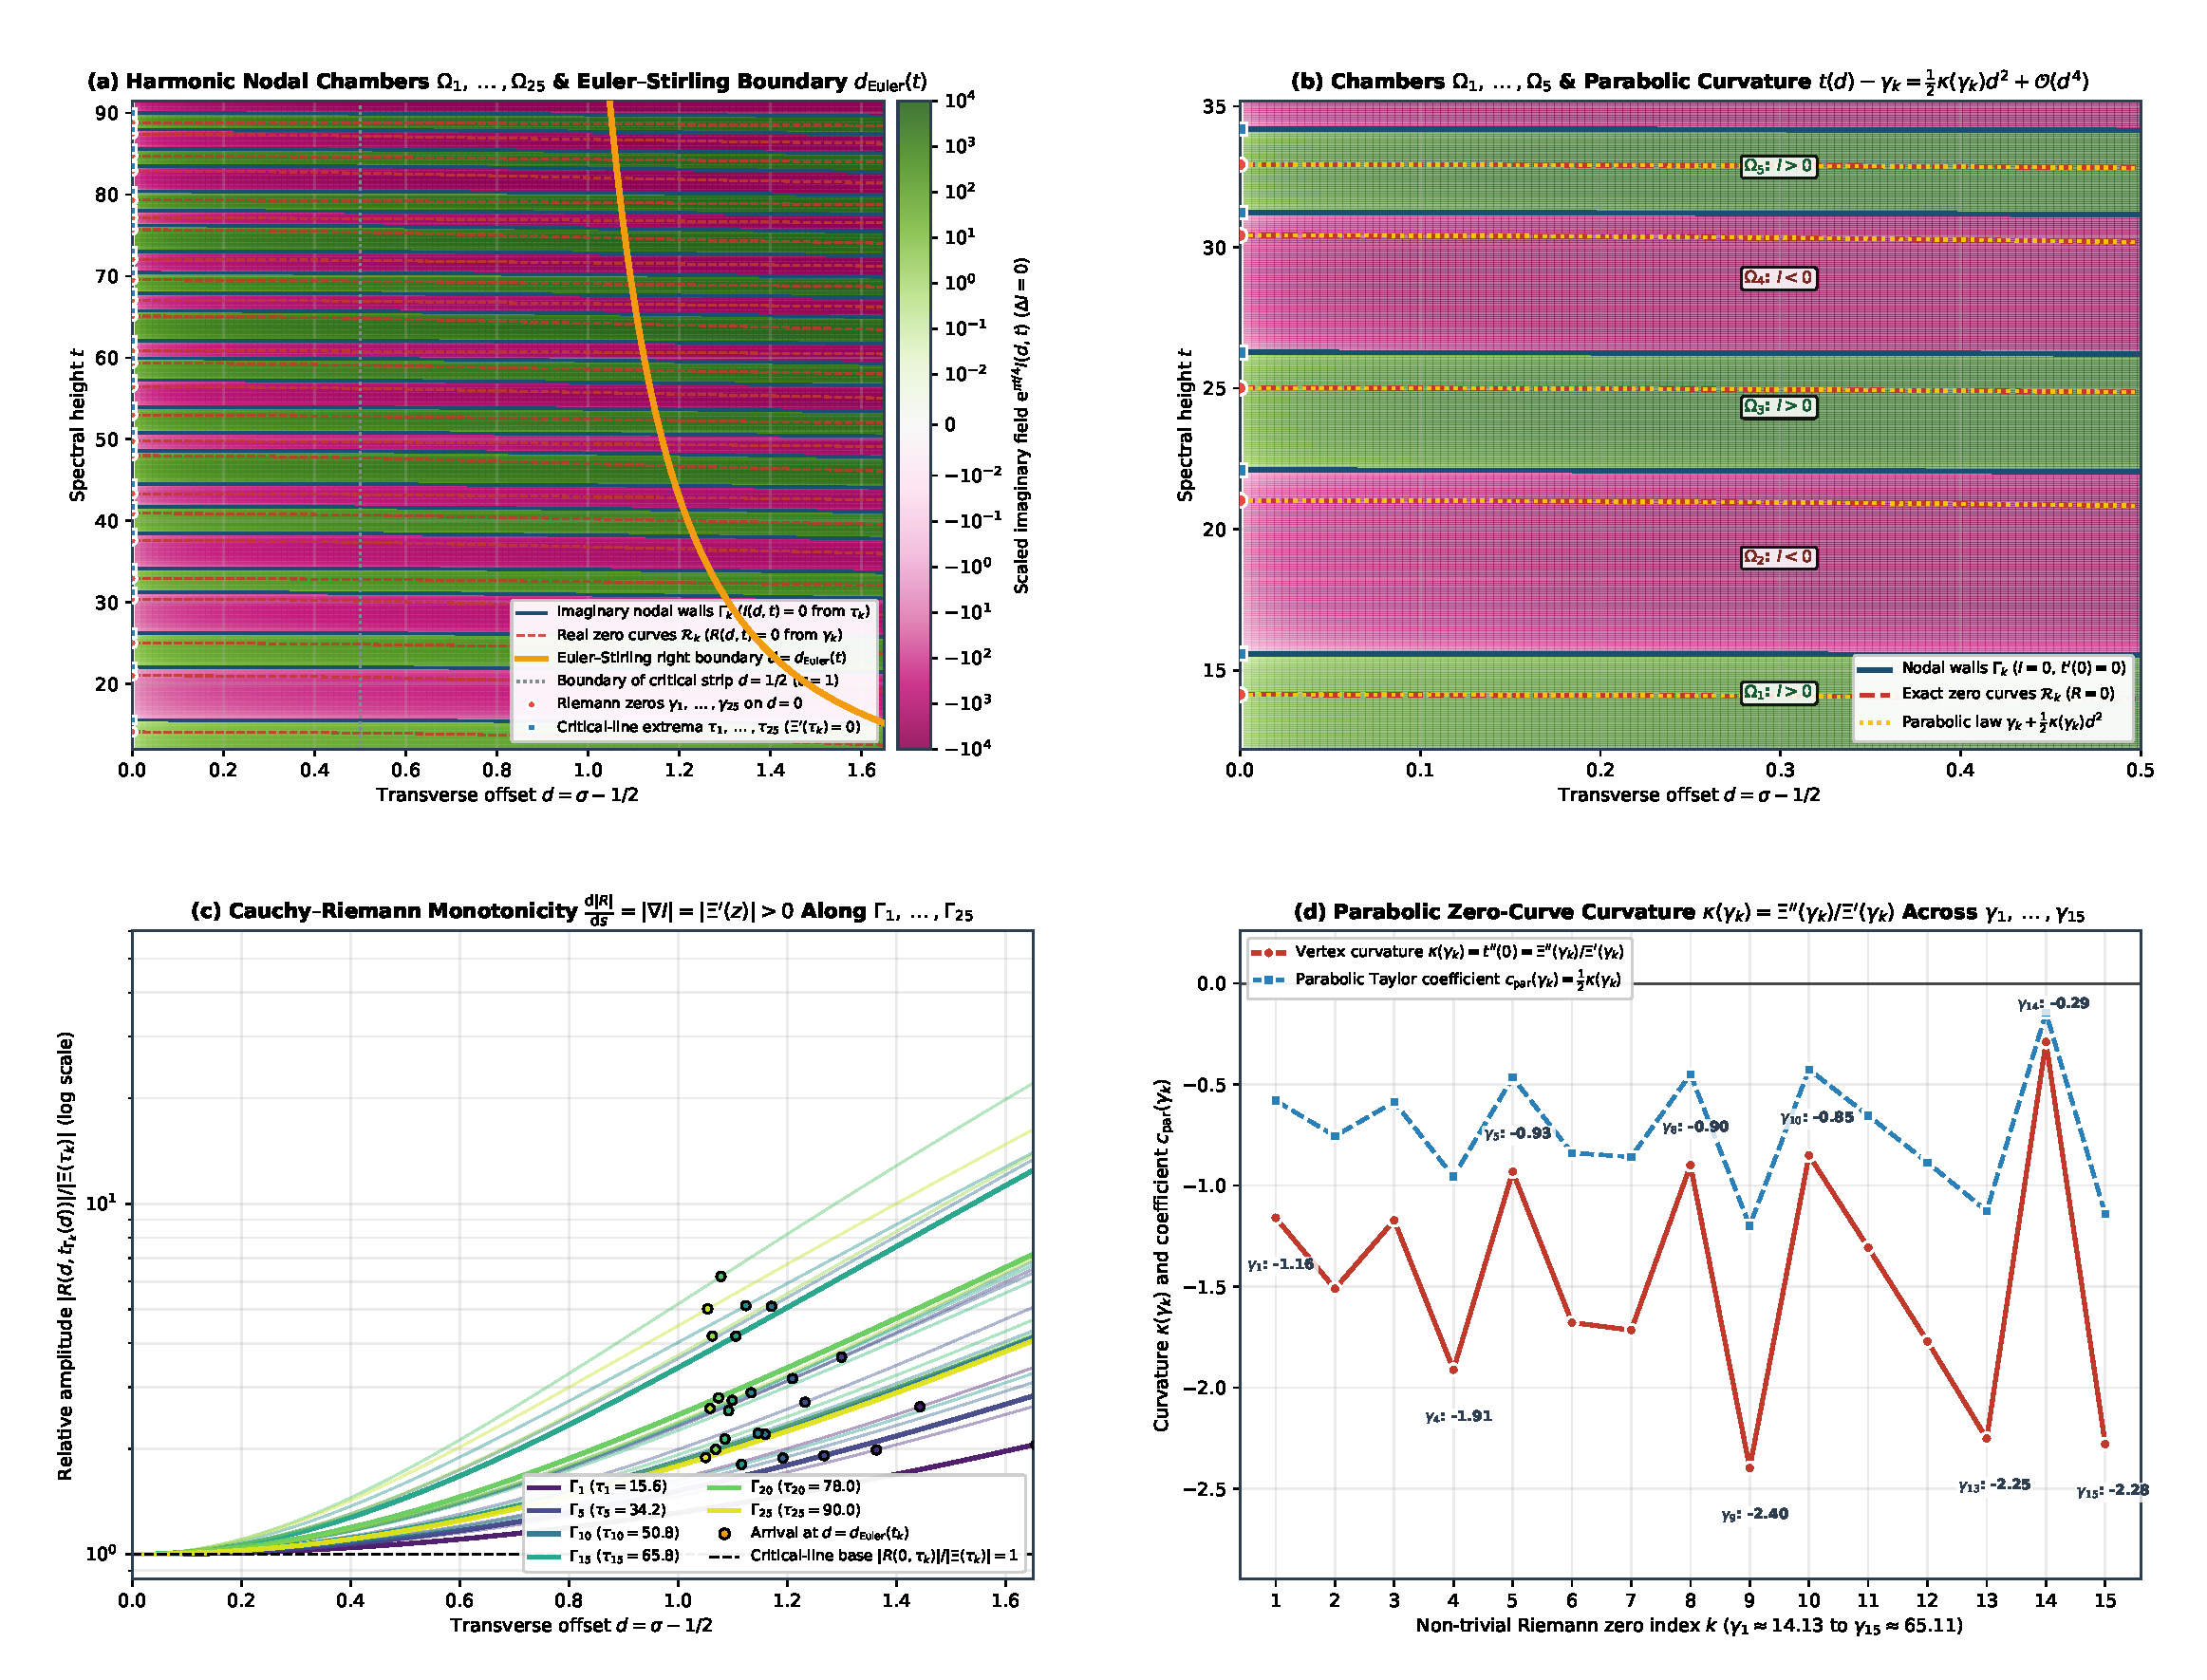
\includegraphics[width=0.95\textwidth]{figures/fig1_harmonic_chladni_chambers_and_curvature.pdf}
\caption{(a) Tracked harmonic nodal chambers $\Omega_1, \dots, \Omega_{25}$ from $d = 0$ across $d = \frac{1}{2}$ ($\sigma = 1$) to the Euler--Stirling boundary $d = d_{\mathrm{Euler}}(t) > \frac{1}{2}$. (b) Close-up of $\Omega_1, \dots, \Omega_5$ showing orthogonal departure of $\Gamma_k$ from $\tau_k$ and agreement between $\mathcal{R}_k$ and $t(d) = \gamma_k + \frac{1}{2}\kappa(\gamma_k)d^2$. (c) Arc-length growth $|R(d,t_{\Gamma_k}(d))|/|\Xi(\tau_k)|$ along $\Gamma_1, \dots, \Gamma_{25}$. (d) Zero-curve curvature $\kappa(\gamma_k) = \Xi''(\gamma_k)/\Xi'(\gamma_k)$ and $c_{\mathrm{par}}(\gamma_k) = \frac{1}{2}\kappa(\gamma_k)$ across $\gamma_1, \dots, \gamma_{15}$.}\label{fig:chambers_curvature}
\end{figure}

\begin{figure}[htbp]
\centering
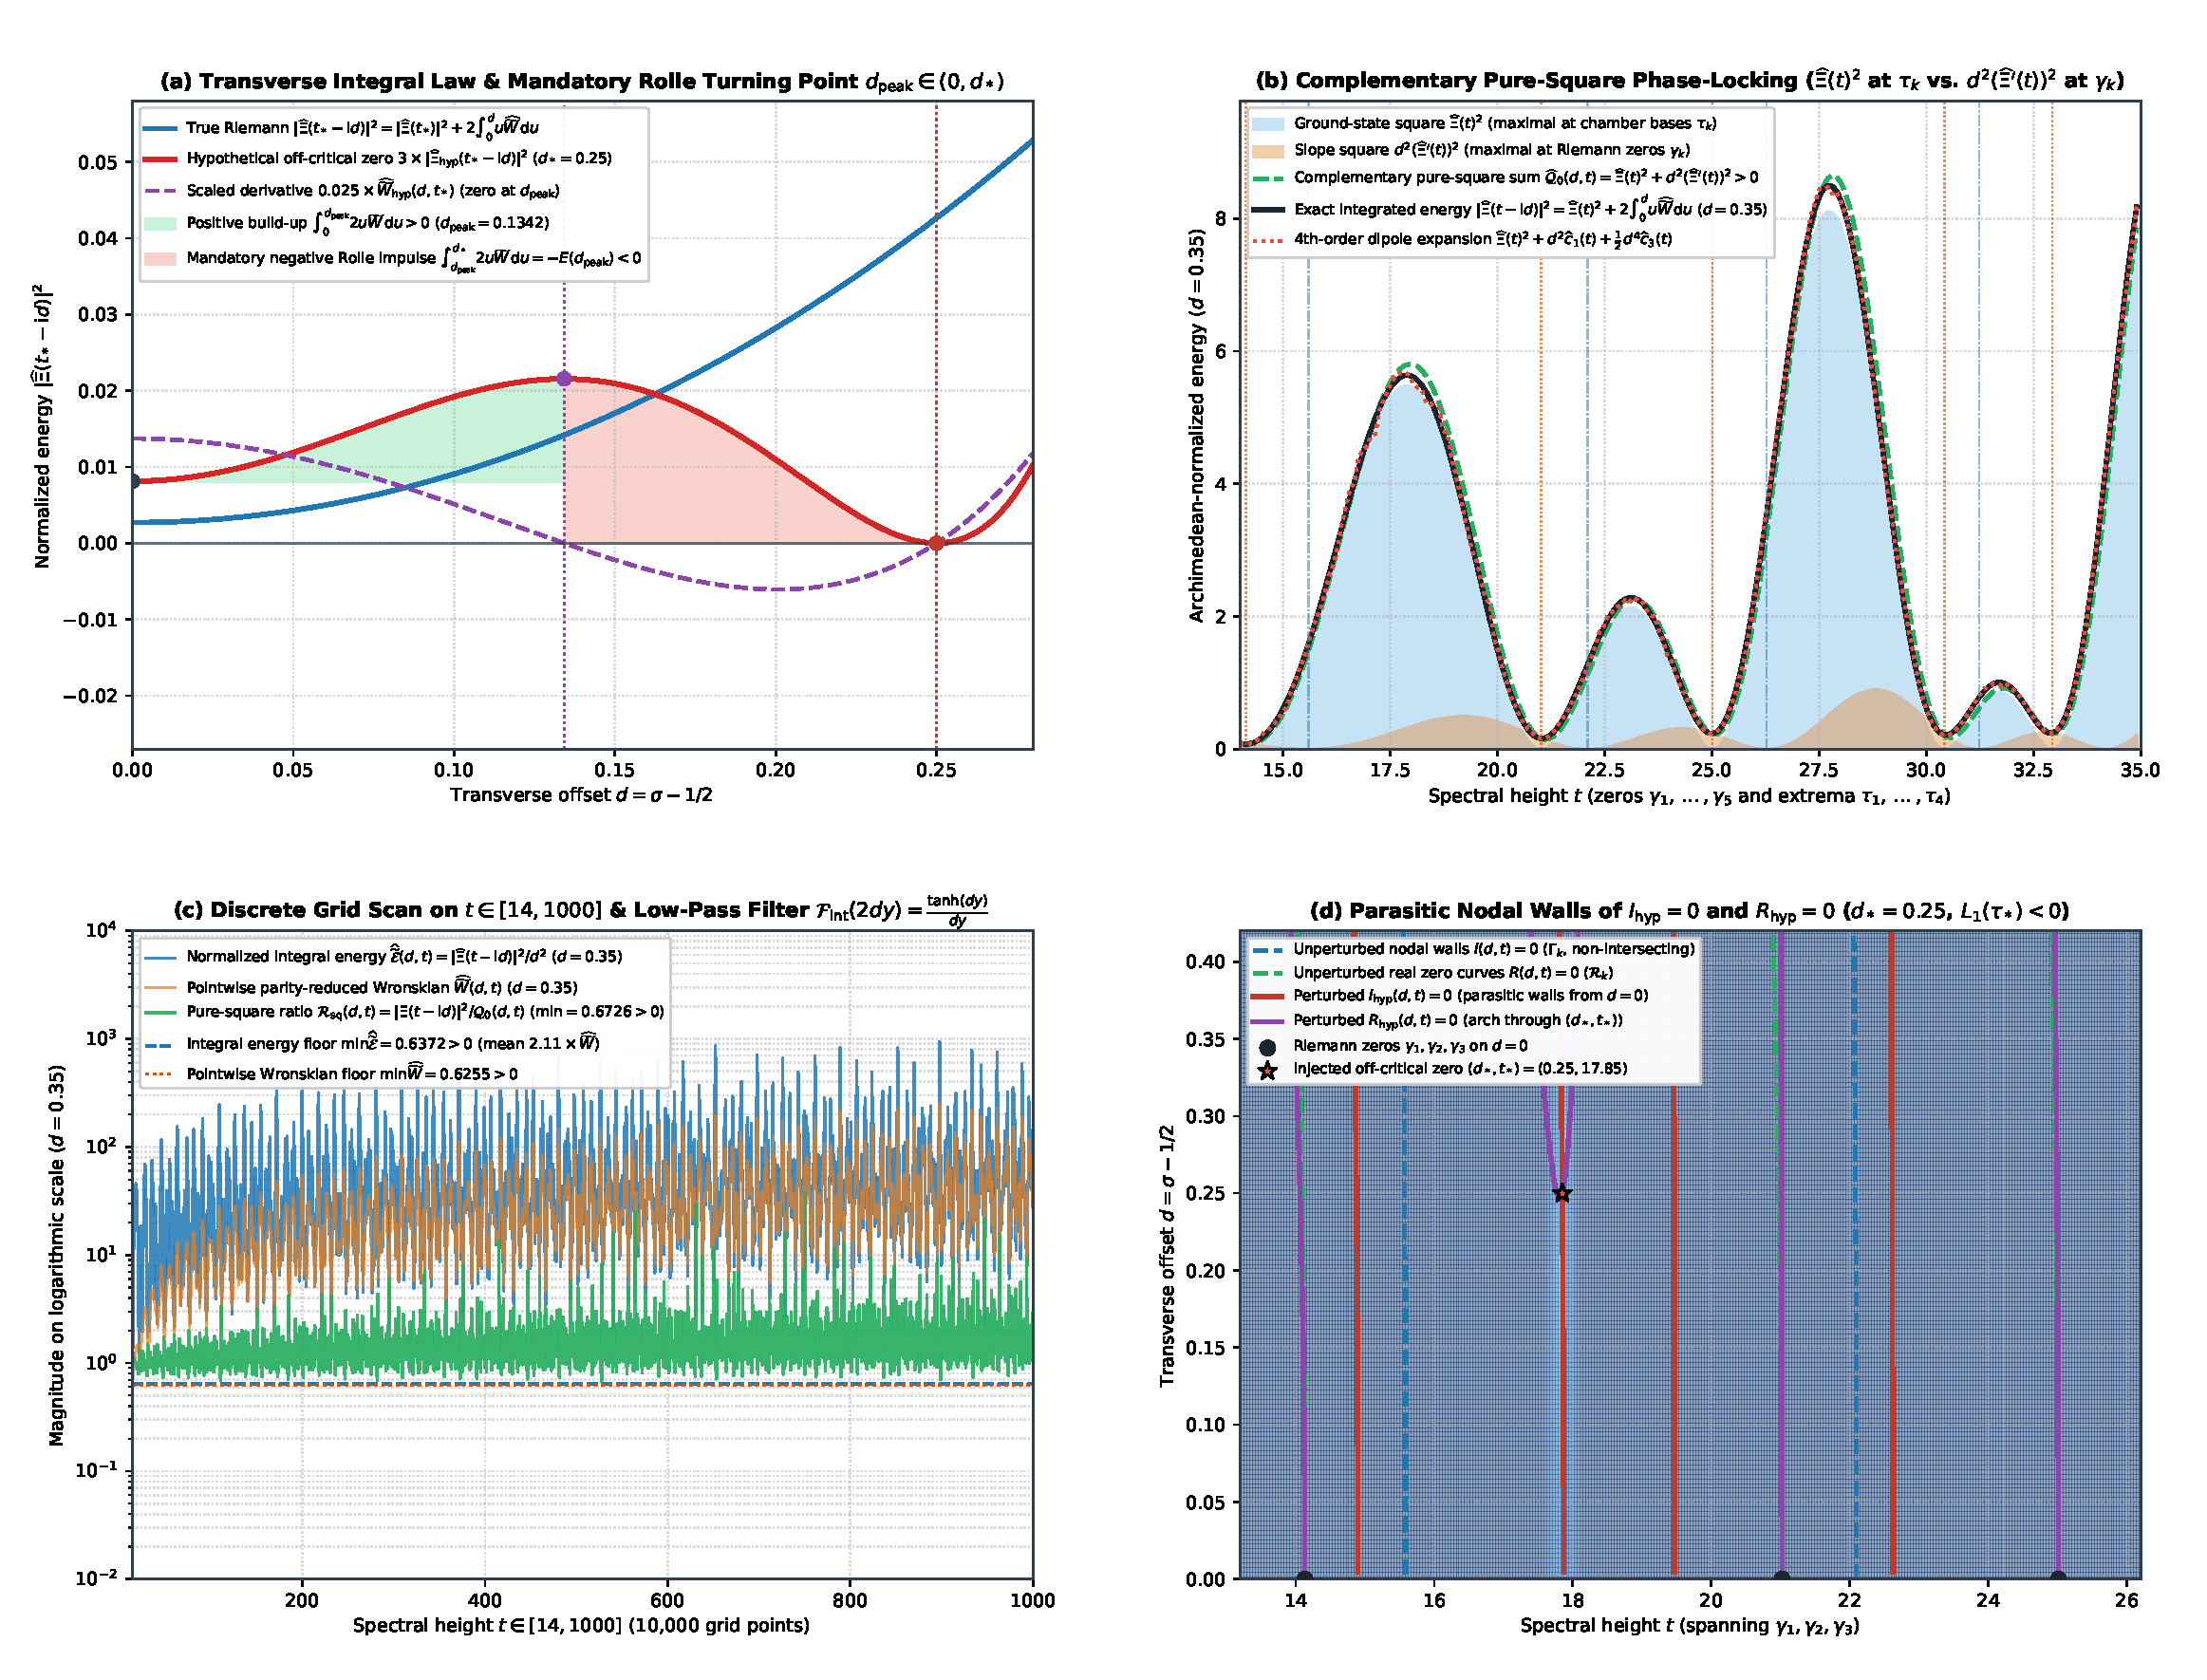
\includegraphics[width=0.95\textwidth]{figures/fig2_transverse_integral_law_and_lowpass.pdf}
\caption{(a) Comparison of $|\widehat{\Xi}(t_*-\ii d)|^2$ against the off-critical perturbation $|\widehat{\Xi}_{\mathrm{hyp}}(t_*-\ii d)|^2$ ($d_* = 0.25, t_* = 14.20$), illustrating the Rolle turning point $d_{\mathrm{peak}} \in (0,d_*)$. (b) Quadrature interleaving of $\widehat{\Xi}(t)^2$ (maximal at $\tau_k$) and $d^2(\widehat{\Xi}'(t))^2$ (maximal at $\gamma_k$) on $t \in [14, 35]$. (c) Discrete grid scan on $t \in [14, 1000]$ at $d = 0.35$. (d) Parasitic nodal walls of $I_{\mathrm{hyp}} = 0$ and arch of $R_{\mathrm{hyp}} = 0$ for $\Xi_{\mathrm{hyp}}(z; 0.25)$, where $L_1(\Xi_{\mathrm{hyp}}; \tau_*) < 0$ on $d = 0$.}\label{fig:integral_lowpass}
\end{figure}

\section{Scope, limitations, and explicit obstructions}\label{sec:scope}

We record the logical scope of our results and the explicit analytical obstructions that prevent harmonic nodal geometry or transverse kernel filtering from yielding an unconditional proof of RH:
\begin{enumerate}
\item \textbf{Circularity of critical-point-free and Laguerre-positivity hypotheses:}
Propositions~\ref{prop:boundary_conditions}, \ref{prop:maximum_and_euler}(a), \ref{prop:dichotomy}, and Theorems~\ref{thm:cr_monotonicity}, \ref{thm:parabolic_curvature}, and~\ref{thm:integral_law_rolle} hold for \emph{any} entire function real on $\mathbb{R}$. To conclude globally that $|R|$ grows along every wall $\Gamma_k$, one must assume both $L_1(\Xi;\tau_k) > 0$ on $d = 0$ and $\Xi'(t-\ii d) \neq 0$ on $d > 0$; by Lagarias \cite{Lagarias1999}, the latter hypothesis is already equivalent to RH.
\item \textbf{The Davenport--Heilbronn obstruction:}
The completed Davenport--Heilbronn function $\Xi_{\mathrm{DH}}(z)$ \cite{DavenportHeilbronn1936,Titchmarsh1986} is entire of order $1$, real on $\mathbb{R}$, symmetric under $s \leftrightarrow 1-s$, harmonic ($\Delta R_{\mathrm{DH}} = \Delta I_{\mathrm{DH}} = 0$), and satisfies the arc-length equation \eqref{eq:dabsR_ds} and the boxed Transverse Integral Identity \eqref{eq:boxed_integral_law}. Nevertheless, lacking an Euler product, $\Xi_{\mathrm{DH}}$ has infinitely many zeros in $d > 0$ (including in $\sigma > 1$), realized geometrically through boundary extrema with $L_1(\Xi_{\mathrm{DH}}; \tau) < 0$ and interior critical points $\Xi_{\mathrm{DH}}'(z_{\mathrm{crit}}) = 0$ per Proposition~\ref{prop:dichotomy}.
\item \textbf{Sign oscillations of $I_{\mathrm{Wig}}(y,t)$ and Lehmer/Skewes phenomena:}
Although Theorem~\ref{thm:lowpass_and_squares}(a) maps $\sinch(2u y)$ into the non-negative square $\sinch^2(d y) \ge 1$ and damps large shifts by $\Fint(2d y) = \frac{\tanh(d y)}{d y} \in (0,1)$, the Wigner correlation kernel $I_{\mathrm{Wig}}(y,t)$ changes sign rapidly with $y$ (exhibiting $5$, $6$, and $7$ sign changes already at $\gamma_3, \gamma_4, \gamma_5$ \cite{Missiaen2026Paper1}). Hence positivity of $\int_0^\infty y^2\sinch^2(d y)I_{\mathrm{Wig}}(y,t)\,\dd y$ cannot be deduced from integrand positivity, and at extreme Lehmer pairs or Skewes-scale phase alignments where $|\Xi'(\gamma_k)|$ is anomalously small, $|\kappa(\gamma_k)|$ becomes arbitrarily large while the baseline square $\mathcal{Q}_0(d,\gamma_k) = d^2(\Xi'(\gamma_k))^2$ becomes arbitrarily small.
\item \textbf{Restriction of $d_{\mathrm{Euler}}(t)$ to $\sigma > 1$ and Voronin universality in $\frac{1}{2} < \sigma < 1$:}
The deductive boundary $d_{\mathrm{Euler}}(t) > \frac{1}{2}$ in Proposition~\ref{prop:maximum_and_euler}(b) lies strictly inside the Euler-product half-plane $\sigma = \frac{1}{2}+d > 1$, approaching $\sigma = 1^+$ only at rate $(\frac{1}{2}\ln t)^{-1}$. Inside the open right half of the critical strip $0 < d < \frac{1}{2}$ ($\frac{1}{2} < \sigma < 1$), the Dirichlet series for $-\zeta'(s)/\zeta(s)$ diverges and Voronin's universality theorem \cite{Voronin1975} implies that $\zeta'(s)/\zeta(s)$ approximates arbitrary complex values on vertical translates, precluding any triangle-inequality majorant of the form \eqref{eq:euler_positivity} for $d < \frac{1}{2}$.
\end{enumerate}

\appendix

\section{Quartic nodal-curve jet and Euler--Stirling asymptotics}\label{app:expansions}

\begin{lemma}[Quartic nodal-curve coefficients and asymptotic expansion of $d_{\mathrm{Euler}}(t)$]\label{lem:app_expansions}
\begin{enumerate}
\item[\textup{(a)}] At any simple real zero $\gamma_k$ ($f(\gamma_k) = 0$, $f'(\gamma_k) \neq 0$) of an entire function $f$ real on $\mathbb{R}$, the fourth-order coefficient $c_{\mathrm{quart}}(\gamma_k) = \frac{1}{24}t_{\mathcal{R}_k}^{(4)}(0)$ in \eqref{eq:t_Rk_expansion} is given by \eqref{eq:kappa_and_cquart}. At any non-degenerate real critical point $\tau_k$ ($f'(\tau_k) = 0$, $f''(\tau_k) \neq 0$), the imaginary nodal curve $\Gamma_k$ satisfies $t_{\Gamma_k}(d) - \tau_k = c_{\mathrm{par},\Gamma}(\tau_k)d^2 + c_{\mathrm{quart},\Gamma}(\tau_k)d^4 + \mathcal{O}(d^6)$ with $c_{\mathrm{par},\Gamma}(\tau_k) = \frac{f'''(\tau_k)}{6f''(\tau_k)}$ and
\begin{equation}\label{eq:cquart_wall}
c_{\mathrm{quart},\Gamma}(\tau_k) = \frac{20\,f^{(4)}(\tau_k)\,c_{\mathrm{par},\Gamma}(\tau_k) - 60\,f'''(\tau_k)\,c_{\mathrm{par},\Gamma}(\tau_k)^2 - f^{(5)}(\tau_k)}{120\,f''(\tau_k)}.
\end{equation}
\item[\textup{(b)}] As $t \to \infty$, the root $d_{\mathrm{Euler}}(t) > \frac{1}{2}$ solving $\mathcal{A}(d, t) = M_{\mathrm{Euler}}(d)$ in Proposition~\ref{prop:maximum_and_euler}(b) satisfies
\begin{equation}\label{eq:d_euler_asymp}
d_{\mathrm{Euler}}(t) = \frac{1}{2} + \frac{1}{\frac{1}{2}\ln\frac{t}{2\pi} + \gamma_{\mathrm{E}} + \mathcal{O}\big((\ln t)^{-1}\big)} \longrightarrow \frac{1}{2}^+,
\end{equation}
where $\gamma_{\mathrm{E}} = 0.5772156649\dots$ is the Euler--Mascheroni constant.
\end{enumerate}
\end{lemma}

\begin{proof}
(a) Truncating \eqref{eq:RI_taylor_d} at $d^4$ gives $R_f(d,t) = f(t) - \frac{1}{2}f''(t)d^2 + \frac{1}{24}f^{(4)}(t)d^4 + \mathcal{O}(d^6) = 0$. Substituting $t = \gamma_k + c_2 d^2 + c_4 d^4 + \mathcal{O}(d^6)$ around $f(\gamma_k) = 0$ yields
\[
\Big[f'(\gamma_k)(c_2 d^2 + c_4 d^4) + \frac{1}{2}f''(\gamma_k)c_2^2 d^4\Big] - \frac{1}{2}\Big[f''(\gamma_k) + f'''(\gamma_k)c_2 d^2\Big]d^2 + \frac{1}{24}f^{(4)}(\gamma_k)d^4 + \mathcal{O}(d^6) = 0.
\]
Matching $d^2$ gives $c_2 = c_{\mathrm{par}}(\gamma_k) = \frac{f''(\gamma_k)}{2f'(\gamma_k)}$, and matching $d^4$ gives $f'(\gamma_k)c_4 + \frac{1}{2}f''(\gamma_k)c_2^2 - \frac{1}{2}f'''(\gamma_k)c_2 + \frac{1}{24}f^{(4)}(\gamma_k) = 0$, proving \eqref{eq:kappa_and_cquart}. Substituting $t = \tau_k + c_{2,\Gamma}d^2 + c_{4,\Gamma}d^4 + \mathcal{O}(d^6)$ into $\widetilde{I}_f(d,t) = -f'(t) + \frac{1}{6}f'''(t)d^2 - \frac{1}{120}f^{(5)}(t)d^4 + \mathcal{O}(d^6) = 0$ similarly yields \eqref{eq:cquart_wall}.

(b) By Stirling's expansion $\psi(z) = \ln z - \frac{1}{2z} + \mathcal{O}(|z|^{-2})$ as $\Ima(z) \to \infty$, $\mathcal{A}(d,t) = \frac{1}{2}\ln\frac{t}{2\pi} + \mathcal{O}(t^{-2})$ uniformly on $d \in [\frac{1}{2}, 2]$. Writing $\sigma = \frac{1}{2}+d = 1 + \varepsilon$ ($\varepsilon > 0$), the Laurent expansion $-\frac{\zeta'(1+\varepsilon)}{\zeta(1+\varepsilon)} = \frac{1}{\varepsilon} - \gamma_{\mathrm{E}} + \mathcal{O}(\varepsilon)$ \cite[Section~2.1]{Titchmarsh1986} gives $\frac{1}{\varepsilon} - \gamma_{\mathrm{E}} + \mathcal{O}(\varepsilon) = \frac{1}{2}\ln\frac{t}{2\pi} + \mathcal{O}(t^{-2})$, proving \eqref{eq:d_euler_asymp}.
\end{proof}

\section*{Use of AI and Computational Tools}

\textbf{Gemini} (Google DeepMind) was used interactively to assist with symbolic manipulations of the fourth-order implicit nodal-curve jets, literature cross-checks, and generation of the \texttt{mpmath}, \texttt{mpmath.iv}, and GPU verification scripts in \nolinkurl{scripts/verify_paper3_harmonic_nodal_chambers.py}. All analytical proofs, interval bounds, and bibliographic references were verified independently.

\begin{thebibliography}{99}

\bibitem{AriasDeReyna2003}
J.~Arias~de~Reyna, \emph{X-ray of Riemann's zeta-function}, Preprint, arXiv:math/0309433 (2003).

\bibitem{Csordas1986}
G.~Csordas, T.~S.~Norfolk, and R.~S.~Varga, \emph{The Riemann hypothesis and the Tur\'an inequalities}, Trans. Amer. Math. Soc. \textbf{296} (1986), no.~2, 521--541.

\bibitem{CsordasSmithVarga1994}
G.~Csordas, W.~Smith, and R.~S.~Varga, \emph{Lehmer pairs of zeros, the de Bruijn--Newman constant $\Lambda$, and the Riemann hypothesis}, Constr. Approx. \textbf{10} (1994), no.~1, 107--129.

\bibitem{CsordasVarga1990}
G.~Csordas and R.~S.~Varga, \emph{Necessary and sufficient conditions and the Riemann hypothesis}, Adv. Appl. Math. \textbf{11} (1990), no.~3, 328--357.

\bibitem{DavenportHeilbronn1936}
H.~Davenport and H.~Heilbronn, \emph{On the zeros of certain Dirichlet series.~I, II}, J. London Math. Soc. \textbf{11} (1936), 181--185, 307--312.

\bibitem{DeBruijn1950}
N.~G.~de~Bruijn, \emph{The roots of trigonometric integrals}, Duke Math. J. \textbf{17} (1950), 197--226.

\bibitem{Gram1903}
J.-P.~Gram, \emph{Note sur les z\'eros de la fonction $\zeta(s)$ de Riemann}, Acta Math. \textbf{27} (1903), 289--304.

\bibitem{Hinkkanen1997}
A.~Hinkkanen, \emph{On functions of bounded type}, Complex Variables Theory Appl. \textbf{34} (1997), no.~1--2, 119--139.

\bibitem{Jensen1913}
J.~L.~W.~V.~Jensen, \emph{Recherches sur la th\'eorie des \'equations}, Acta Math. \textbf{36} (1913), 181--195.

\bibitem{Lagarias1999}
J.~C.~Lagarias, \emph{On a positivity property of the Riemann $\xi$-function}, Acta Arith. \textbf{89} (1999), no.~3, 217--234.

\bibitem{Lehmer1956}
D.~H.~Lehmer, \emph{Extended computation of the Riemann zeta-function}, Mathematika \textbf{3} (1956), 102--108.

\bibitem{Missiaen2026Paper1}
T.~Missiaen, \emph{Wigner Phase-Space Representation, Shifted Cauchy Contours, and Local Saddle-Point Coalescence in the Transverse Wronskian of Riemann's $\Xi$-Function}, Preprint, Zenodo (2026), DOI: \href{https://doi.org/10.5281/zenodo.23637324}{10.5281/zenodo.23637324}.

\bibitem{Missiaen2026Paper2}
T.~Missiaen, \emph{Parity-Reduced Transverse Wronskians, Jensen--Laguerre Moment Identities, and Division-Free Interval Enclosures for Riemann's $\Xi$-Function}, Preprint, Zenodo (2026), DOI: \href{https://doi.org/10.5281/zenodo.23641698}{10.5281/zenodo.23641698}.

\bibitem{Newman1976}
C.~M.~Newman, \emph{Fourier transforms with only real zeros}, Proc. Amer. Math. Soc. \textbf{61} (1976), no.~2, 245--251.

\bibitem{PlattTrudgian2021}
D.~J.~Platt and T.~S.~Trudgian, \emph{The Riemann hypothesis is true up to $3\cdot 10^{12}$}, Bull. Lond. Math. Soc. \textbf{53} (2021), no.~3, 792--797.

\bibitem{Polya1926}
G.~P\'olya, \emph{Bemerkung \"uber die Integraldarstellung der Riemannschen $\xi$-Funktion}, Acta Math. \textbf{48} (1926), 305--317.

\bibitem{Polya1927}
G.~P\'olya, \emph{\"Uber die algebraisch-funktionentheoretischen Untersuchungen von J.~L.~W.~V.~Jensen}, Kgl. Danske Vid. Sel. Math.-Fys. Medd. \textbf{7} (1927), no.~17, 3--33.

\bibitem{Riemann1859}
B.~Riemann, \emph{Ueber die Anzahl der Primzahlen unter einer gegebenen Gr\"osse}, Monatsberichte der Berliner Akademie (1859), 671--680.

\bibitem{RodgersTao2020}
B.~Rodgers and T.~Tao, \emph{The De Bruijn--Newman constant is non-negative}, Forum Math. Pi \textbf{8} (2020), e6, 1--62.

\bibitem{Speiser1934}
A.~Speiser, \emph{Geometrisches zur Riemannschen Zetafunktion}, Math. Ann. \textbf{110} (1934), no.~1, 514--521.

\bibitem{Spira1965}
R.~Spira, \emph{Zero-free regions of $\zeta^{(k)}(s)$}, J. London Math. Soc. \textbf{40} (1965), 677--682.

\bibitem{Spira1968}
R.~Spira, \emph{Zeros of $\zeta'(s)$ in the critical strip}, Math. Comp. \textbf{22} (1968), 163--173.

\bibitem{Spira1973}
R.~Spira, \emph{Zeros of $\zeta'(s)$ and the Riemann hypothesis}, Illinois J. Math. \textbf{17} (1973), 147--152.

\bibitem{Titchmarsh1986}
E.~C.~Titchmarsh, \emph{The Theory of the Riemann Zeta-Function}, 2nd ed., edited and with a preface by D.~R.~Heath-Brown, Oxford University Press, Oxford, 1986.

\bibitem{TitchmarshComrie1936}
E.~C.~Titchmarsh, \emph{The zeros of the Riemann zeta-function}, Proc. Roy. Soc. London Ser. A \textbf{151} (1935), 234--255; \textbf{157} (1936), 261--263.

\bibitem{Voronin1975}
S.~M.~Voronin, \emph{Theorem on the ``universality'' of the Riemann zeta-function}, Math. USSR-Izv. \textbf{9} (1975), no.~3, 443--453.

\bibitem{Wigner1932}
E.~Wigner, \emph{On the quantum correction for thermodynamic equilibrium}, Phys. Rev. \textbf{40} (1932), 749--759.

\end{thebibliography}

\end{document}
